\documentclass[11pt,oneside]{report} 
\usepackage{geometry}                		
\geometry{letterpaper}                   		
\usepackage{graphicx}					
\usepackage{amssymb}
\usepackage{multirow}
\usepackage{comment}
\usepackage[natbibapa]{apacite}
\usepackage[table,xcdraw]{xcolor}
\usepackage[T1]{fontenc}
\usepackage{booktabs}
\newcommand{\ra}[1]{\renewcommand{\arraystretch}{#1}}
\usepackage{tabularx}
\usepackage{fontspec}


\linespread{1.3}

\usepackage{lmodern}

\usepackage[hidelinks]{hyperref}
\usepackage{color}
\usepackage[font={footnotesize}]{caption}
\usepackage{subcaption}


\usepackage[framemethod=tikz]{mdframed} %Adds control over nice customisable text boxes
\usepackage{enumitem} %Adds customisation of item lists
\usepackage{pifont} %Adds access to special chars like the ones I use in the chapter summary boxes
\usepackage{framed} %Adds the frame support

%Create a new element - the chapter summary box
\newmdenv[
%shadow=true,
%leftline=false,
%rightline=false,
linewidth=1pt,
\setmainfont{Gill Sans MT},
innertopmargin=10pt,
innerbottommargin=20pt,
innerrightmargin=20pt,
]{mynote}

\begin{document}
%\setmainfont{Gill Sans MT}
%%%%%%%%%%%%%%%%%%%%%%%%%%%%%%%%%%%%%%%%%
% University Assignment Title Page 
% LaTeX Template
%
% This template is made and modified by Judith Borghouts based on a template downloaded from:
% http://www.latextemplates.com
%
% Original author:
% WikiBooks (http://en.wikibooks.org/wiki/LaTeX/Title_Creation)
% 
% Instructions for using this template:
% This title page is presently capable of being compiled as is. This is not 
% useful for including it in another document. To do this, you have two options: 
%
% 1) Copy/paste everything between \begin{document} and \end{document} 
% starting at \begin{titlepage} and paste this into another LaTeX file where you 
% want your title page.
% OR
% 2) Remove everything outside the \begin{titlepage} and \end{titlepage} and 
% move this file to the same directory as the LaTeX file you wish to add it to. 
% Then add \input{./title_page_1.tex} to your LaTeX file where you want your
% title page.
%
%%%%%%%%%%%%%%%%%%%%%%%%%%%%%%%%%%%%%%%%%

%----------------------------------------------------------------------------------------
%	PACKAGES AND OTHER DOCUMENT CONFIGURATIONS
%----------------------------------------------------------------------------------------


%\begin{document}

\begin{titlepage}

\newcommand{\HRule}{\rule{\linewidth}{0.5mm}} % Defines a new command for the horizontal lines, change thickness here

\center % Center everything on the page


%----------------------------------------------------------------------------------------
%	TITLE SECTION
%----------------------------------------------------------------------------------------

\HRule \\[0.4cm]
{\Large \bfseries Understanding how people look up and enter data in financial office settings
}\\[0.4cm] % Title of your document
\HRule \\[1.5cm]
 
%----------------------------------------------------------------------------------------
%	AUTHOR SECTION
%----------------------------------------------------------------------------------------

\begin{minipage}{0.4\textwidth}
\begin{flushleft} \large
\emph{Author:}\\
Judith \textsc{Borghouts} % Your name
\end{flushleft}
\end{minipage}
~
\begin{minipage}{0.4\textwidth}
\begin{flushright} \large
\emph{Supervisors:} \\
Dr. Duncan \textsc{Brumby} \\% Supervisor's Name
Dr. Anna \textsc{Cox}
\end{flushright}
\end{minipage}\\[4cm]

% If you don't want a supervisor, uncomment the two lines below and remove the section above
%\Large \emph{Author:}\\
%John \textsc{Smith}\\[3cm] % Your name

%----------------------------------------------------------------------------------------
%	DATE SECTION
%----------------------------------------------------------------------------------------

{\large \today}\\[3cm] % Date, change the \today to a set date if you want to be precise

%----------------------------------------------------------------------------------------
%	WORD COUNT
%----------------------------------------------------------------------------------------

%Word count: 23081 as counted by detex dissertation.tex $ | $ wc -w

%This includes the report and appendices.

\begin{minipage}{0.4\textwidth}
\begin{center}
UCL Interaction Centre,\\
Department of Psychology, \\
University College London
\end{center}
\end{minipage}
~

\vfill % Fill the rest of the page with whitespace

%----------------------------------------------------------------------------------------
%	HEADING SECTIONS
%----------------------------------------------------------------------------------------

%\textsc{\LARGE University of York}\\[1.5cm] % Name of your university/college
\begin{flushright} \large

\includegraphics[width=\textwidth]{images/logo.pdf}%\\[1cm]  % Include a department/university logo - this will require the graphicx package
\end{flushright}
%\textsc{\Large Department of Computer Science
%}\\[0.5cm] % Major heading such as course name

%\textsc{ Submitted in part fulfilment of the degree of the requirements for the degree of:}\\[0.5cm] % Minor heading such as course title

 
%----------------------------------------------------------------------------------------




\end{titlepage}
%\end{document}

\begin{abstract}

When people have to perform data entry tasks such as entering expenses, this involves retrieving data from one or more sources in the environment and entering it into a computer system. Switching between entering data and looking up the required data can be disruptive, as people have to pay a time cost each time they resume their data entry task. Furthermore, the cost to access these sources may vary, which can further influence the disruptiveness of looking up the information. In order to design interfaces that support people in their data entry work, it is therefore important to understand how these differences in access affect switching behaviour between entering and retrieving data. 

This thesis investigates how information access costs (IAC) affect how people manage subtasks of looking up information for a data entry task. Six studies are reported across three chapters, to understand the impact of IAC in the context of entering expenses in a finance office setting.

The first part of the thesis reports a series of qualitative studies that look at the context in which office workers in financial offices perform data entry tasks.  For entering expenses, people often had to go out of the data entry system to look up information. A planned study aims to further investigate the information sources needed for this task and their IAC, and the strategies people currently use to retrieve information from these sources.

The second part of the thesis reports a series of quantitative studies that investigate the extent to which observed behaviour of the first studies are due to the access costs of the information sources involved. When people copy from one source and IAC increases, people make fewer switches to look at this source, and instead enter what they have memorised. This makes people more efficient, but slightly increases errors. A planned study aims to further investigate switching behaviour when people have to retrieve the information from multiple sources.

The final part of the thesis then reports two studies that explore if design interventions can make people adopt more desirable strategies, i.e. strategies that minimise switching between entering data and looking up the required data. 

The primary contribution of this thesis is to show the fragmented nature of an expenses task, and that the IAC of required information sources affects how people manage how they look up certain information, which in turns impacts accuracy and efficiency. This finding has implications for the design of the current expenses system, which are validated through demonstration of how changing certain design features can potentially better support people in managing these subtasks of looking up information for a data entry task.

\end{abstract}

\fboxsep=10pt
\fboxrule=0.5pt

\tableofcontents
\listoffigures
\listoftables
\chapter{Introduction}

\begin{mynote}
\subsubsection{Chapter outline}
In this chapter, I outline the problem I am addressing in this thesis, and the proposed contribution.
\end{mynote}

\vspace{10pt}
 
Imagine, you have come back from a business trip and have to claim back your expenses. You open the expenses system and enter the first few personal details such as your name from the top of your head without any problem. For the expenses you want to claim back, you get up to collect your receipts from your wallet and start entering the items and prices into the system. The prices are in a foreign currency, so you leave the expenses system to go to a currency converter website and convert the prices. You then need to enter your account number. You go and get your wallet with bank cards from your bag. How many times have you stopped entering to go and look up certain information? Or did you get all the required information beforehand, so you did not have to get up in-between? You may have entered the information you knew first, and left the remaining items until the end? Whatever way you chose to complete the task, it involved making decisions on how to manage subtasks of looking up the required information for the entry task. 

Data entry is usually a straightforward task, but when information has to be retrieved from multiple sources, not all of which are as easy to access, this simple task can quickly become complex. Switching between entering data and looking up the required data can be disruptive, as you have to pay a time cost 
each time you resume your data entry task. You may have forgotten where you were, enter information in the wrong place, or misremember what you were supposed to enter and enter something incorrect. This disruption can introduce data entry errors, the outcomes of which can range from annoying to more serious consequences, such as transferring money to the wrong bank account, or transferring a wrong amount.  

Because it is important data entry is done accurately, data entry research has looked at improving the input interfaces \citep[e.g.][]{Oladimeji2013, Vertanen2015, Wiseman2013a}, but it is not clear its design implications generalise to the type of situation as described above. In this situation, you do not enter all items from a source nearby, as in most data entry studies, but need to retrieve and enter different types of information (e.g. numbers, alphanumeric strings, words) from multiple sources (e.g. e-mails, paper receipts, different computer windows). The cost to access these resources varies, and if information becomes harder to access, people increasingly rely on what they have memorised of the information rather than recheck the resource \citep{Gray2006}. It is however not known how people prioritise and manage their tasks when they have to retrieve the information from multiple resources, with varying access costs, or how a data entry interface should be designed to support people in these situations. 

While it has been shown how changing the design of a data entry interface can affect and improve how we enter data, and that different information access costs affect how often people consult one source, it is not known how the interface can support situations when data has to be retrieved and entered from various sources with varying information access costs. In order to design interactive systems that truly support this type of data entry task, it is necessary to get a detailed understanding of how users manage this task and its subtasks, and to what extent the access to the required resources affect their strategies.

This thesis investigates how different information access costs affect how people manage subtasks of looking up information for a data entry task, with the aim to inform the design of data entry systems. 
In order to design systems that truly support the task they are intended for, it is necessary to get a detailed understanding of this task. 
For the scope of this thesis, I look specifically at how employees in financial administration offices manage looking up information from various sources for an expenses task. This task requires entering different types of information from a variety of sources, such as paper, spreadsheets, emails and databases. It is important the task is done accurately but within a reasonable amount of time as they are under time pressure to finish work on time. This data entry task is therefore considered to be an appropriate and interesting example to study further. 

The expenses task serves as an example of a wider class of data entry tasks, and it can be imagined findings of this thesis can be useful and generalise to other, similar, tasks. For example, people who have to fill in their tax returns have to similarly enter a range of information into a computer system, and have to collect this information from multiple sources with varying IACs.

The research questions of this thesis are:

\begin{enumerate}
\item Does the IAC of information sources affect how people manage subtasks to look up information for an expenses task in a finance office setting?
\begin{enumerate}
\item	What (types of) information do people need for entering expenses?
\item	Where do people need information from?
\item	How do they address those needs?
\item	Does the type of information, and where they need it from, affect how people address these needs?
\end{enumerate}
\item	How can the existing data entry system be redesigned to support or better support people managing subtasks of looking up information for entering expenses, given variable IACs for required information sources?
\end{enumerate}


The first contribution of this thesis is to map out the fragmented nature of an expenses task, of which looking up information is a substantial part of the task. It investigates how the information access cost of required information sources affects how people manage when they look up certain information. This finding has implications for the design of the current system: a second contribution is demonstrating how changing certain design features can better support people in managing these subtasks of looking up information.



\chapter{Background}\label{ch:Background}

\begin{mynote}
%\vspace{0.5cm}
\subsubsection{Chapter outline}
In this chapter, I review previous literature on which I build my research on expenses tasks in a financial office setting. The first half of the chapter will focus on the data entry task, and how certain design changes can influence people's speed and accuracy. The second half of the chapter will focus on the setting, and discuss challenges of performing tasks in an office environment.
%\vspace{0.2cm}
\end{mynote}

\section{Data entry}
A data entry task can be broken down in four stages (see Figure \ref{fig:ch2_hip}). An information source contains the input, i.e. the data to be entered. In the perception stage, the user perceives this data. In the encoding stage, the user encodes these in the mind. In the execution stage, the user enters them into a device which produces the output of the task, namely the data entered. Additionally, there can be a checking stage where the user checks their entered output against the original input to see if it matches.

\begin{figure}[!ht]
\centering
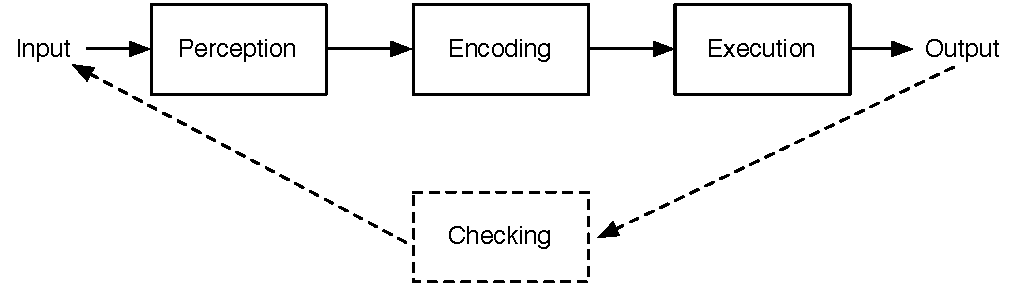
\includegraphics[width=0.8\textwidth]{images/HIP.pdf}
\caption[Different stages of a data entry task]{The different stages of a routine data entry task: a user perceives data input, encodes these in the mind, executes certain actions to enter data and produce the output, and can check the output against the original input.}
\vspace{-3pt}
\label{fig:ch2_hip}
\end{figure}

The following four sections will describe each stage of the task in turn, and will discuss research that has been done to reduce errors at this stage. 
Throughout this thesis the terms data, text, and number entry are used. If data is used, this refers to alphabetic, alphanumeric, and numeric characters. 
If the term text is used and no particular clarification is given, this refers to alphabetic text. If numbers are discussed and no specification is given, this refers to the Arabic notation of numbers, in other words digits. 

\subsection{The perception stage}
A data entry task begins with the user looking at the data that has to be entered on a data source.
Both the design of the data source as well as the data itself can ultimately have an influence on task performance. In this section, I will describe the following themes: the distribution of internal and external cognition, external representations, the memorability of data, and how presenting data in a disfluent manner can influence people's cognitive encoding of the information.

\subsubsection{Distributed cognition}
When people perform a task, they can make use of information in their mind, or retrieve information from the external environment \citep{Norman1993}.
The distributed cognition approach has been used as a theoretical framework to explain how people make use of internal and external information to carry out work \citep{Hollan2000}. In contrast with traditional cognitive science approaches that take the individual mind at the center of analysis, distributed cognition explains how the completion of a task is determined by one or more users interacting with each other, their environment, as well as external artefacts \citep{Hutchins1995}. The framework suggests that external representations are not merely a memory aid to off-load the limited capacity of someone's working memory, but form an integral part of cognition. In other words, it is not only the amount of external information, but also its format that can considerably affect performance \citep{Gong2009, Zhang2009}.
To be able to understand how people work, it is not enough to know how the mind processes information but it is also important to know how the information is arranged in the physical world \citep{Hollan2000}. 

\citet{Payne2013} argue that some proponents of distributed cognition assume people off-load as much cognition to external resources as possible. However, as will be discussed in section \ref{sec:Encoding_stage}, the decisions people make on whether to offload or not is better understood as adaptive, and is affected by context as well as the design of the interface or artefacts. 

\subsubsection{External representations}
Building on the work that external representations are part of cognition and that their format influence how people process and understand information, work has been carried out to explore different ways to represent information to the user. 

An important factor in designing appropriate external representations is to consider how users currently use these representations. \citet{Hutchins1995} gives a case study of cockpits as an example, in which the dial to indicate airspeed was replaced with a more precise digital display. This design did not take pilots into consideration, and only after interviews was it revealed that the new display did not match with how pilots made use of this external information. Pilots did not think of the speed as a number, but used the spatial structure of a dial to perceive their current speed and its proximity to the desired speed. By replacing the dial with digits, they lost this information. 

With a better understanding of how people use representations in a certain context, these representations can also be organised in a way to make people adapt to more desirable strategies. \citet{Back2013b} looked at programming infusion pumps in hospitals, where it is best practice to program each pump one by one, rather than interleaving in-between pumps. They found that the visual organisation of information on charts can encourage this best practice: if numeric values belonging to one pump were grouped together, participants were more likely to first finish programming one pump, before they started programming another pump.

\subsubsection{Memorability of data}
People's performance in copying data is not only influenced by how the data is organised on the source, but also by the data itself.
From text entry, it is known that words are easier to transcribe than non-words as they are more meaningful and thus have a stronger representation in memory \citep{Salthouse1986}. Based on this, \citet{Wiseman2014} investigated if the same was true for numbers. Experiments showed that familiar numbers are faster to transcribe, suggesting that these are more strongly represented in memory than random numbers as well.
An applied example is PIN numbers, which is usually entered very quickly at around two seconds and at a low error rate \citep{DeLuca2010}. In this case, both the digits as well as the unique motor movements made across the keypad are well encoded in memory \citep{Mangen2010}. 

In order to make numbers in a transcription task easier to memorise and check for errors, \citet{Sandnes2013} explored how numbers could be represented as words instead, based on the assumption that words are easier to remember and are easier to check for errors. 
In this paper, she presented a fixed dictionary with 100,000 numbers, each of which had a word associated with it. 
Instead of reading and typing the number, the user would read and type in the word that belongs to it, and a computer system would identify the corresponding number. 
Words would be easier to remember than a string of digits, and it would also be easier for a system to establish if an error is likely, when a word is typed that is not found in the dictionary. This novel way of presenting numbers can reduce cognitive load on the user and catch errors, but may not always be applicable depending on the domain. Numbers can be a random sequence of digits such as a phone number, but they may also have a specific meaning, such as in the financial and medical domain where a number can represent a a financial amount or medication volume.
By abstracting the numbers and representing them as words that bear no relation with the meaning of the number, users do not have a sense anymore of the meaning of the numbers they are copying, which may not always be desirable.

\subsubsection{Presenting data in a disfluent manner}
The strength of information in memory can influence people's performance on copying that information, and users are both faster and more accurate in copying familiar words and numbers, rather than abstract strings of characters. If however the data to copy is abstract to the user, and cannot easily be changed or mapped onto a familiar word or other representation, there are still other ways to encourage people to encode data more deeply. 

Designers of information sheets may intuitively try to present information in a way that is easy to perceive for the user, but some studies have shown that making information more difficult to perceive can have a positive effect.
\citet{Diemand-Yauman2011} presented text in a grey and hard-to-read font, and found this aided people in processing and understanding the text better than when the text was presented in a normal font. The idea behind this study was that a hard-to-read font forced people to make more of an effort to read and understand the text, and as a result the text was more deeply processed and encoded in the mind. Building on this study, \citet{Soboczenski2013} conducted two studies where people had to transcribe text and numbers that were presented either in a black font colour or a harder-to-read grey font colour. Participants made fewer data transcription errors if data was shown in the harder-to-read font colour, both for transcribing text and numbers. There was no difference in speed between the hard-to-read and normal font colour, suggesting that the improved accuracy was not due to a speed-accuracy trade-off. This is an important finding because it shows that a deeper encoding of information may not only be beneficial when understanding text, but also when information has to be transcribed. It also shows that changing the representation can influence the encoding strategies people adopt.
Further work is needed to see if this effect will remain over time, as people may either get used to the font and the effect will weaken, or people may become frustrated. 

\subsubsection{Summary}
The first part of the data entry task entails the user perceiving the input.  A stronger representation of data in memory can improve task performance. Data may be strongly presented in memory because the data to enter is familiar to the user, but the design of the input source can also influence people's cognitive strategies and encourage a deeper encoding. Both internal and external information affect task performance, and where and how input is presented in the external environment affects people's internal representation of it. 

\subsection{The encoding stage}\label{sec:Encoding_stage}
After the user has perceived the input source in a data entry task, the next stage in the task sequence is the encoding stage, where data is encoded in memory. In this section, I will discuss how the cost to access information, and the effect of writing versus typing, affects how people encode information.

\subsubsection{Information access cost}
When the user perceives data, the effort involved to encode this data into memory can be influenced by the design of the data source, but also by the ease with which the source can physically be accessed in the environment. The time, physical and/or mental effort required to access information is called information access cost (IAC), and increases in the cost to access information are intrinsic to everyday tasks \citep{Morgan2009, Waldron2011}. In order to view information needed for a task, people may have to open and reopen documents, go back to a previous page, have to switch attention between their device and paper sheets, use different screens, and often have to use and retrieve information from different sources. If information is permanently available, people adopt a display-based strategy and rely on the external display as memory source. As it becomes harder to access information however, it will take too much time to retain a display-based strategy, and people will be more likely to switch to a memory-based strategy and commit more information to memory to minimise going back and forth to this external information.

This adaptive use of memory is explained by the soft constraints hypothesis, which holds that people adapt their cognitive strategies to the constraints of a task environment with the aim to optimise task completion time \citep{Gray2006}. The hypothesis states that rather than minimising cognitive resources, people try to minimise time. 

To test the robustness of the hypothesis, the effect of IAC has been tested in lab experiments on several tasks such as copying tasks \citep[e.g.][]{Gray2006}, problem solving tasks\citep[e.g.][]{Morgan2012}, and flight simulation tasks \citep{Waldron2007}. A consistent finding is that people adapt their strategies to the ease with which information can be retrieved in the environment.  A memory-based strategy may be faster rather than looking up the external information, but it carries the risk that the memorised items are incorrect. \citet{Gray2006} therefore recommend that the effort it costs to access information should be kept low. Similarly, \citet{Kohn2000} advise that designers of interactive devices should not rely on weak aspects of human beings, such as working memory.

However, several studies have shown that an increased IAC can have a positive effect. In problem-solving tasks, an increased IAC resulted in people taking the time to memorise task information and more planning behaviour before making any moves, which made them more efficient in completing the task \citep[e.g.][]{Morgan2007, Morgan2012}. 

A memory-intensive strategy can also be useful for resuming a task after an interruption. Task interruptions are known to be disruptive, because it takes time to resume the task and it can increase errors \citep{Back2010, Brumby2013, Morgan2009}. 
\citet{Morgan2009} conducted a study looking at the effect of IAC on a copying task. People had to perform the Blocks World Task (BWT), which involves copying a pattern of coloured blocks, by dragging blocks from a resource window to a target window. They manipulated the cost to access the original source which showed the pattern they had to copy. In the Low IAC condition, the pattern was permanently visible on the screen. In the Medium IAC condition, the pattern was covered by a grey mask and participants had to hover over the mask with their mouse to reveal the pattern. In the High IAC condition, there was an additional time delay before the pattern was revealed. At certain intervals, they would get interrupted and asked to do a secondary task. As IAC increased, people made fewer but longer visits to the target pattern and memorised more of the pattern. As a result, following an interruption they were faster to resume and could copy more blocks before having to revisit the target pattern. 

In an experiment by \citet{Brumby2013}, people had to perform a data entry task and were interrupted several times to do a secondary task. They manipulated the cost of making an error and if the cost was high, an error would cause the participant to be locked out for 10 seconds before they could resume the primary task. In this condition, people took a longer time to resume, but were less likely to make errors. A lockout made people adopt a memory-intensive strategy and take the time to remember where they were in the sequence before resuming the task. 

\citet{Back2012} studied the programming of two infusion pumps, and the numbers participants had to enter were situated either next to the pumps or 50 cm away. If the numbers were next to the pumps, participants saw them as individual numbers which caused them to interleave more in between the two pumps and make more errors. 
However, when the numbers were further away, people grouped the numbers, and first entered all numbers of one pump, and then entered the numbers of the second pump. This strategy caused them to make fewer errors. 

These studies show that a memory-based strategy can be beneficial for task performance, but only if people make the effort to encode the information and therefore have the correct information in the mind. In a data entry task, it is therefore important to know what a person is reliably able to keep in short-term memory and copy correctly at once. This information can be used to design interfaces in a way that if people choose to adopt a memory-intensive strategy, they should be encouraged to check back to external information at certain times and not try to memorise too much.

\subsubsection{The effect of writing versus typing on the level of encoding}
The design of, and access to, the data source can influence how deeply people encode data in memory. In addition, the way we execute entering or transcribing the data can influence how deeply we encode it. \citet{Mangen2010} argue there is a strong relation of cognitive processing of information and the motoric movements we have to make to input that information, and the hand movements we make to type can influence how deeply we process the information we are inputting. 

\citet{Mueller2014} looked at note-taking amongst university students, and found that students retained more information when they made notes by hand, rather than by laptop. Participants were asked to attend a talk and make notes.
The talk and exams were not part of the students' curriculum and did not count towards their final grade but were set up to resemble a typical lecture and exam: the talk was followed in a lecture theatre at their university and the content was similar to what they studied. 
After the talk, the students then were presented with distractor tasks. 
\citet{Mueller2014} conducted one study where participants were tested straight after the distractor tasks and a second study where participants were examined after one week. 
In both studies, participants who made notes by hand scored significantly higher on the exams. The authors support their findings with the encoding hypothesis, which holds that the processing that occurs during note-taking influences learning and retention of learning material.  Participants who took notes with laptops were more inclined to take verbatim notes and made more notes, but the information was transcribed without a deeper processing of the information that was typed. 
Furthermore, because it took more time to write something down versus typing it, people took the time to think about what to write down and remembered this better.

While the task of taking notes during a lecture is different from data entry, some things can be taken from this study that may be applied to data entry as well. 
People who have to transcribe a lot of data via a conventional keyboard may switch to automatic processing in the same way as people who take notes with laptops. Though it is unfeasible to let people transcribe data by hand in most data entry situations, it does indicate how slowing people down or applying unique movements to certain characters, instead of using the same buttons that give the same haptic feedback, may promote encoding.

\subsubsection{Summary}
At the second stage of the data entry task, the user processes the input in the mind. While usually designers aim to make it easy for people and not put too much cognitive load on the user, in some cases making the user process the information more deeply and adopt a memory-intensive strategy can have a positive effect on task performance. In the case of an interruption, taking time to remember where people were in the task sequence can reduce resumption errors. Furthermore, a deep encoding of data in memory can make people more accurate in data entry.

\subsection{The execution stage}
The third stage of the data entry task is the execution stage, which is the stage where the user performs the motoric actions to enter data into a device.

\citet{Reason1990} makes a distinction between two types of errors: slips and mistakes. Mistakes happen when we enter what we have in our mind accurately, but we have the wrong thing in mind. Changing the data source can influence the level of encoding users engage in to prevent these mistakes. However, even when we have the right thing in mind, we can still enter it inaccurately, which is called a slip. In order to prevent these errors from happening, work has been done on changing the entry interface. This section gives an overview of current research on both text and number entry, and how these two forms of data entry are similar and different.

\subsubsection{Text entry}
Two primary metrics in measuring people's performance on a data entry task are speed and accuracy. These metrics are commonly understood as being trade-offs: an increase in typing speed will come at the cost of errors, and a focus on entering data accurately will come at a time cost \citep{MacKenzie2002, Smith2008}.  While ideally a user should perform well on both metrics, in some situations one metric can be more important than the other. In text entry, the focus has typically been on improving entry speed while remaining an acceptable accuracy.

Two popular methods in text entry to improve performance are movement minimisation and text prediction \citep{MacKenzie2002}. With movement minimisation, the movements of the fingers to type in text are minimised. In text prediction, the system predicts the words the user intends to enter based on typed characters so far and completes the word. An alternative method is text correction, where the system waits until a user has typed a word and then tries to detect and correct errors. This relieves users from the task to check their input, and lets them concentrate on typing. \citet{Vertanen2015} created a touch screen keyboard for mobile devices called VelociTap, which used sentence-based correction instead of word-based correction. This meant people entered a full sentence before the system tried to correct input. Experiments showed that this type of text correction significantly reduced error rate while not affecting entry rate compared to a normal touch screen phone keyboard. The correction allowed users to be able to concentrate on entering text until the end of a sentence, and they were not distracted by words being predicted or corrected after each word. Furthermore, it allowed the system to take the context of words within a sentence in account and was more accurate in determining what the correct words should be.

\subsubsection{Number entry}
Text and number entry follow the same stages outlined in Figure \ref{fig:ch2_hip}. As with text entry, number entry involves the user looking at a number, encoding this, and entering it into a device. There are however some aspects in which number entry is different, which is why findings from text entry research cannot always be directly applied to number entry.
 
For instance, text prediction or correction is hard to apply to number entry because as opposed to text, there is no dictionary to determine if a number is correct or not \citep{Wiseman2013a}, making it hard to predict what the user intends to type. In some settings however there are certain numbers that are inputted more often than others. \citet{Wiseman2013a} looked at number entry in hospitals and found clear patterns in the numbers being entered. In a study building on this, \citet{Wiseman2013b} made adaptations to existing interfaces to make it easier to type in commonly used numbers in hospitals. Fewer key presses were needed to type in common numbers and as a result numbers were typed in faster, without an increase in the error rate. This shows number entry interfaces can and should be tailored to the numbers that people have to enter. 

\citet{Healy2004} looked at how performance on a number entry task changes over time. They conducted an experiment in which participants were asked to enter 640 four-digit numbers, and observed both learning and fatigue-like effects. People became faster, but also increasingly less accurate in entering numbers. The authors suggest this may be because fatigued participants switch from controlled to automatic processing where they no longer deeply encode the numbers they are entering. To reduce fatigue effects, they conducted a second experiment where halfway through the experiment participants switched hands to type in the numbers. Despite this switch, the same increase in speed and errors was shown, and the authors suggest the the major cause of fatigue in data entry was cognitive rather than motoric, as a switch in hands should be more effective to muscular fatigue than attentional fatigue. It could also be the case that people became bored and wanted to be done with the task, as there was no incentive to perform well. However, while people became faster overall in entering numbers, their initiation time increased, which means that people took a longer time at the start of each number before they started entering it. \citet{Healy2004} suggests this is another indication of cognitive fatigue. 
The authors recommend trainees in data entry work should be warned about losing accuracy over time, and should be instructed to respond more slowly. 

The speed with which users enter data can be influenced by the design of the input method. \citet{Oladimeji2011} compared a number keypad with an incremental interface. The two types of interfaces are shown in Figure \ref{fig:interface-styles}. The number keypad is most common, and is used on calculators and phones. In this interface, each digit is assigned a button and additional buttons are usually a decimal point and a delete key to correct an error, as shown in Figure \ref{fig:numberpad}. In an incremental interface, a number is entered by increasing or decreasing the number using up and down keys. The incremental interface used in \citeauthor{Oladimeji2011}'s study is shown in Figure \ref{fig:incremental}. The double arrows increase and decrease the number by a larger amount than the single arrows.

\begin{figure}[]
\begin{center}

\begin{subfigure}[b]{0.3\textwidth}
\centerline{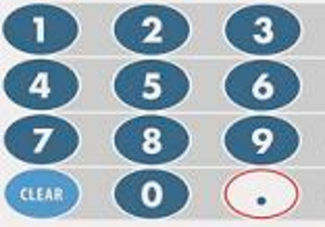
\includegraphics[scale=0.8]{images/numberpad.pdf}}
\caption{A number pad.}
\label{fig:numberpad}
\end{subfigure}
%\hfill%
\begin{subfigure}[b]{0.5\textwidth}
\centerline{
\includegraphics[scale=0.5]{images/incremental.pdf}}
\caption{An incremental interface.}
\label{fig:incremental}
\end{subfigure}

\caption[An incremental and keypad number entry interface.]{Two different number entry interfaces tested in \citeauthor{Oladimeji2011}'s study.}

\label{fig:interface-styles}
\end{center}
\end{figure}

Results of the study showed that a number keypad allowed people to enter a number more quickly than an incremental interface, but more errors were made. With the keypad, the visual attention was more on the input keys than the display. In an incremental interface, people were changing an existing value rather than entering a new value, so they had to look at the display to see how their actions changed the current value. This attention on the display may have made it more likely for them to detect errors in time. While an incremental interface may not be feasible when entering large amounts of data as it will slow users down too much, it may be preferrable over a keypad in situations where accuracy is of great importance \citep{Thimbleby2011}. 

In order to reduce human data entry errors, attempts have also been made to eliminate the need to manually enter data altogether. This is however not always possible, and moreover can introduce different problems.
\citet{Koppel2008} studied medication bags with a scannable bar code to enter numbers, so that the numeric values did not have to be typed by a person. They identified 31 workarounds if the system failed, for example if the bar code was missing, blurry or when the scanner did not work properly. Furthermore, even with a scanner numbers still have to be entered manually at some point, and it abstracts the numbers, which means users do not have a sense anymore of the magnitude of the numbers they are copying \citep{Wiseman2013a}. 

\subsubsection{Summary}
At the third stage of the data entry task, the user inputs the data into a device. Data entry has a speed-accuracy tradeoff, and being able to enter data faster often come at the cost of an increased error rate. 
Keyboards that slow people down may be useful in cases where accuracy is important, but may not be feasible in situations where a lot of data has to be entered. Depending on what users have to enter, shortcuts may get introduced in keyboard design so commonly used data can be entered quicker without the cost of increased errors. 

\subsection{The checking stage}
Most data transcription models consider the execution stage as the final stage of a data entry task \citep{Card1983, Salthouse1986}, but an additional stage can be a checking stage, where people review their entered output and compare it with the original target input, to see if it matches. 
In addition to studies trying to prevent errors before they occur, other studies have taken a different approach and looked at how a user can detect and correct errors after they have occurred. 

\subsubsection{Double data entry}
A number of studies have compared two or more of the following error checking techniques in data entry: visual checking, read aloud, and double data entry \citep{Barchard2011, Barchard2013, Kawado2003}. In visual checking, the user visually compares the entered data with the original data. In read aloud, data from the original source is read out loud by one user and the entries are visually checked by another user. In double data entry, data is entered twice and cross-checked by the computer system. 

Overall, double data entry is shown to be the most effective method in detecting errors. This method is often used in online forms when a user has to enter a password or e-mail address twice. The reasoning is that it is unlikely the same mistake is made twice. It is also not necessary for a system to know the correct input beforehand to determine if an entry error is made or not, because the two entries are cross-checked and if they do not match, an error has been made. 
 A disadvantage of double entry is that it requires double labour and can be time-consuming. Double data entry may therefore not be feasible for each setting. 
For example, \citet{Kawado2003} looked at copying medical data, and in their study 104,720 data entry fields had to be entered twice by two different people. In this study, the total times for double data entry was 74.8 hours while for the read aloud, where one person said the numbers and another person entered them, it was 57.9 hours. In situations where a lot of data has to be entered, such as data entry clerk work, it may therefore not be feasible to have to enter all data twice.  Moreover, it is still possible that a mistake is repeated, even when the entry is done by two different people \citep{Nakata2014}. In \citeauthor{Kawado2003}'s (2003) study, 42 errors remained undetected with the double data entry method.

\subsubsection{Visual checking}
Another method to detect errors is for the users to visually check their entered data with the original data source. Visual checking is a popular method \citep{Tu2014}, but simply asking or relying on people to check is often ineffective \citep{Barchard2011, Nakata2014, Norman2002, Olsen2008}. It is particularly hard to visually check numeric data, because there is no top-down error detection: almost any order of digits is a legal number \citep{Lin2014, Nakata2014}. Users can use the context of a word to detect if it is invalid, for example when 'wrod' is typed instead of 'word'. For numbers, if 697 is typed instead of 679 this may be harder to visually spot because 697 still counts as a valid number. 

\citet{Wiseman2013a} looked at a number entry task, and used a checksum to detect number entry errors. This is an extra number, that is related to the other entered numbers in a way that it is sufficient to only check the checksum to determine if the input is correct, instead of checking each entry one by one. 
They used infusion pump parameters in their study, and users were asked to enter the medication volume to be infused and the rate of infusion. If these two numbers were entered, the computer could calculate how long the infusion would take, and this time was the third checksum number.
If the checksum was generated by the computer from the two numbers entered and this checksum had to be visually checked by the user, only 36\% of the errors were caught. If the third number had to be entered by the user as well, and it was checked by the computer against the other two numbers, all errors were caught but the time to complete the task was increased by 46\%. These results show that visual checking was ineffective, but that asking the user to enter extra data can cause a considerable amount of time.

\citet{Olsen2008} conducted a lab experiment in which he simulated an internet banking tool, and participants were asked to enter account numbers from a paper sheet into a computer. After participants had entered an account number, they were presented with a confirmation screen with the input, and users were asked to check their input on this screen before submitting. 
Participants confirmed 88 trials where they had entered an incorrect account number. In addition, in 178 trials the simulator changed people's input to another number and this incorrect number was presented on the confirmation screen. Only 5 of these 178 errors were detected and corrected. This large amount of incorrect confirmations again suggests users do not check properly, even if they are explicitly asked to do so. 

\subsubsection{Lockouts}
Given the limited effectiveness of confirmation screens \citep{Norman2002, Olsen2008}, some studies have supplemented these with lockouts, where users have to wait a short period of time before they are able to confirm and submit their input. 

\citet{Green2014} introduced a lockout in a patient order entry system in a hospital. Every time a physician made an order for a patient, a prompt appeared asking to double-check the identity of the patient, and the button to continue an order would be disabled for 2.5 seconds. The prompt reduced the error rate by 30\%, but the total time to complete ordering tasks was lengthened by 1.5 hours on average. 

\citet{Gould2015} studied a number entry task where after each number the submit button would be disabled for a number of seconds, and a text instruction to check input appeared on the input screen.  This lockout was an effective method in encouraging people to check and detect errors in a lab setting. When the study was replicated online, a short lockout made people detect errors as well but the longer the lockout duration was, the more likely people were to switch to doing other tasks, and not check anymore. This illustrates the importance of taking the task context into account, and that findings from controlled studies do not always directly translate to an applied setting. In situations where people are able to work on other tasks, a lockout has to be brief to be effective and not induce switching to other tasks \citep{Gould2015}. 

Similar switching behaviour was found by \citet{Katidioti2013}. They conducted a lab experiment where people had to copy information and were interrupted by chat messages. Participants were free to choose when they wanted to attend to the messages. When people were locked out in the copying task and had to wait 3 seconds before they could enter the information, they often switched to the chat message, which made them forget the information to copy and slowed them down in completing the task.

\subsubsection{Incentives}
Instead of making design changes to the interface, \citet{Li2015} investigated if people can be motivated to check by incentives. 
They conducted a data entry experiment and manipulated the compensation people received after the experiment. In one condition, participants received extra money if they completed the task error-free. In another condition, money was deducted from their compensation if they made an error. In the control condition they received the same compensation regardless of their performance. Adding rewards and punishments significantly changed people's checking behaviour: they made more frequent and longer checks when their payment depended on their performance, and this resulted in fewer errors. 

\subsubsection{Summary}
After people have entered input, they can choose to check if what they have entered is correct. A popular method is visual checking, but people are poor at doing this, even if they are instructed to do so. It is possible to have people check, but the context needs to be considered. A lockout helped people check, but when possible to switch to other tasks people used the time to spend time on other tasks.

\section{Office work}
The previous section described the different stages of the data entry task, and how changing the data entry interface can influence people's strategies, accuracy and speed. Challenges of data entry in office settings is that data can be fragmented across documents, applications, and tasks: people deal with an increasing amount of information which they need for the task, they have to manage multiple tasks and often interrupt or get interrupted of doing their primary task. This second part of the literature review gives an overview of work that has been done to meet these challenges of working in an office environment. 

\subsection{Reducing information access costs: multiple and larger screens}
Most computer applications are designed to support a part of a task, but do not consider that users may have to use multiple applications for the same activity \citep{Cangiano2009}. Several studies on office workers have found that information work often does not happen within one application or document, but can be highly fragmented \citep{Cangiano2009, Czerwinski2004, Mark2005, Sellberg2014}. People have to go in and out of several applications \citep{Cangiano2009, Iqbal2007}, switch between tasks \citep{Czerwinski2004, Mark2005}, and have to coordinate information distributed over paper files, electronic databases, e-mails, as well as people \citep{Sellberg2014}. 

Office workers change their main work activity on average once every 11 minutes \citep{Mark2005}, and reportedly switch between tasks 50 times over one work week \citep{Czerwinski2004}.  Users can leave the primary task interface because they are distracted by a notification or because they deliberately decide to switch to a completely other task, but can also leave to look up task-relevant information.  The subtask of looking up information is relevant to the primary task so may not always be labelled as an interruption from the main activity, but resuming the primary task of entering information can still be difficult \citep{Rule2013}.

Office workers are dealing with an increasing amount of information, and may have to leave the task interface frequently to look up information. As discussed earlier, hiding information and increasing access costs may have a positive effect, as people encode the information better in memory. They do not need to look up the information as frequently and are more efficient in completing the task \citep[e.g.][]{Waldron2011}. Having the information well-memorised can also make people more robust against interruptions \citep{Morgan2009} and showing data in a harder-to-read font can make people more accurate in text and number transcription tasks \citep{Soboczenski2013}.

In these studies the information to hold in memory was limited and came from one source. When dealing with a lot of information from multiple sources, decisions on what has to be presented where and in what manner is still a challenge and it is often up to users to arrange the required resources for the task \citep{Bardram2006, Grudin2001}.

Flipping back and forth between several documents can make you lose train of thought, and when interrupted you may have forgotten the original intention of what you intended to look up \citep{Grudin2001}.  In order to help people manage information and minimise switching between windows, both multiple and larger screens have been introduced into the workplace. While a number of studies have favoured one large screen over two smaller ones \citep[e.g.][]{Bi2009}, the two solutions seem to have different benefits.

\citet{Bi2009} conducted a study comparing people's behaviour in office work when they had to use one small screen, two small screen, and one large screen. People arranged information on their available screen space differently in each condition. For two screens, people dedicated one screen for their primary task which filled up the entire screen. They moved all information they did not need at the moment to the second screen and did not bother re-arranging the windows: they would only attend to the second screen when they needed information, and deliberately allocated the second screen for a different purpose than the first screen. For one large screen, participants first spent a certain amount of time optimising the layout of the windows by resizing and re-arranging them. They put all windows needed for the primary task in the center of the screen and placed other windows in the periphery.  As participants needed information from this periphery, they dragged the window to the center of the screen rather than interacting with that particular part of the screen. On the other hand, if participants needed information from the second screen, they physically turned to the second screen and interacted with it but did not drag the information to the primary screen, unless they had to interact with it for a longer time.  

For the majority of tasks, participants preferred one large screen over two screens, as it made them feel more immersed in, and surrounded by, their work. Two screens had a physical distance between them, so large documents could not easily be seen across the screens. A further drawback from having two screens was that it needed more physical space on a desk. \citet{Bi2009}  mentioned that a large screen made people better able to monitor other applications during work, such as emails. This was viewed by the authors as a benefit, but may also be more distracting. If such applications are instead placed on a second screen, people will be less disrupted by them because their visual attention is not there, but they can still easily glance at it to see if there are any new notifications \citep{Grudin2001}.  

Despite the popularity of one large screen, \citet{Grudin2001} states dividing screen space up in multiple monitors can sometimes be better. He argued that the main benefit of having a second screen is not so much the increase in screen space, but the partitioning of information into dedicated areas. He compares screen size with a house: sometimes it is better to have two rooms rather than one big room, as you can use the rooms for different purposes, such as one for a bedroom and one for a living room. Similarly, having multiple screens prompts people to think more about where to put which information. To support his argument, he conducted a field study looking at how office workers use multiple screens to arrange information. Participants positioned information they did not need at the moment on a second screen where they were not distracted by it, but could easily access it when needed. People preferred that information was always in the same known location and referred to the second screen whenever they needed to look information up, even when they were aware they could also access it using their primary screen as well, where the information was sometimes less time-consuming to access \citep{Grudin2001}. 

A larger screen can better support people in multitasking, as people will not need to flick back and forth between windows as often, but can have these open and on the screen simultaneously \citep{Czerwinski2003}. However, it can also have a snowball effect: as screen size increases, so does the number of open windows, and people engage in more complex multitasking \citep{Robertson2005}. In addition, a large screen may reduce having to click and tab between windows but it can introduce another type of access cost, which \citet{Robertson2005} refer to as the \textit{'distal information access cost problem'}: as screen size increases, it becomes harder and more time-consuming to target and select certain buttons and windows. 

\subsubsection{Summary}
Office workers deal with an increasing amount of information and it is challenging to decide how to present information needed for the task. An increased screen size can reduce certain access costs, such as mouse clicks to flick back and forth between windows, but may introduce other access costs, such as time to select the right window. 
Multiple and larger screens both increase screen space, but people adopt different behaviour and strategies for each set-up. Two monitors makes people dedicate a second screen for all information sources and secondary tasks, so they can focus their attention on one screen. When using one large screen, people will re-arrange windows to have more windows open at the same time and focus on the primary task but still be aware of other windows. 

\subsection{Managing information needs}
Increased screen space allows people to have more windows open at once. This may reduce the need for people to open and close windows and hold information in memory when flicking between windows, but the responsibility stills lies with the user to first collect and organise all the required resources for the task \citep{Bardram2006}. Some task management applications have been built to support users to collect and group information needed for the task, but people often do not know the complete context of their activity yet and the information they will need. In addition, manually categorising and grouping task-related information can be time-consuming \citep{Cangiano2009}.

People do not always realise they need certain information until they have started a task. Leaving the primary task interface to look up this information does not have to be bad if it is useful for the current activity, but resuming the primary task after this interruption still takes time \citep{Rule2013}.
\citet{Sohn2008} conducted a diary study to get an insight in people's information needs on mobile phones and how they address these needs. They did not focus on a particular task, but asked participants to keep a record of all instances where they needed information for an activity they were doing.

The information needed was retrieved from both public and personal sources on their mobile phones, such as website and e-mails, as well as physical locations. Four main factors determined whether participants looked up the information when they needed it, when they addressed it later or when they did not address it at all: urgency, importance, cost, and situational factors. The more urgent and important it was to have the information for the activity they were doing, the more likely it was they looked up the information at the moment they realised they needed it. The more time or monetary cost was associated with getting the information, the more likely they were to not address it or leave it until later. Other reasons for looking it up later or not at all, was that they were currently involved in an activity that made it difficult to address the information need at that moment, or they did not know where to get the information from.

People sometimes had to switch between several information sources and applications for one task, such as personal e-mails, search engines, and Google Maps. The more effort and time it took to go in and out of these several sources, the more likely it was that the participant gave up on looking up the information at that moment and deferred it until later. The source where people needed to get the information from, and how costly it was to access this source, also influenced whether people looked up information as they needed it or not.

The authors conclude mobile devices should take into account the activity people are doing to make sure information related to a task becomes easy to access. Though it may be difficult to predict which information will be needed, it should be at least easier for users to switch between different information sources.

The information needs in this study were primarily for personal rather than work activities, and people may be less flexible in deciding to not look up information at all when it is work-related. They may however decide to look up information later, and if it is costly to access information or depending on importance of accuracy or efficiency, decide to rely on information they have memorised rather than looking up the information of an external source. 

\subsubsection{Summary}
Office work can be highly fragmented, and people have to go in and out of several documents, applications and windows for the same activity. It is often up to the user to collect information, and it should be made easier for people to collect information for a task and resume it when they leave the primary task interface to look up information. The cost to access information, the urgency and importance of an information need, and the current situation people are in influences their decision on whether they look up information as they need it or not. 

\section{Conclusion}
Data entry follows four stages, and there are multiple strategies to complete the task, some being more accurate or efficient than others. Studies have shown that changing the design of a data entry interface can affect and improve how we enter data, and that different information access costs affect how often people visit the source from which to look up and enter data.

It is not known yet how these data entry designs can be used in an office setting, where people have to manage multiple information sources with varying information access costs. Studies on office work have shown that work can be highly fragmented, and that people may often have to go in and out of several applications to complete their task. 
In order to design interactive systems that truly support this type of data entry task, it is necessary to get a detailed understanding of the task in this setting, how users manage subtasks of looking up information for the data entry task, and to what extent the costs to access required resources affect their strategies.

\chapter{Entering expenses in a financial setting}\label{ch:Study1}
\begin{mynote}
\subsubsection{Chapter outline}

In this chapter I describe the findings of an explorative interview study about data entry in a financial work setting. The aim of this study was to get a better understanding of the type of data entry task people at finance offices conduct, and the physical environment in which this is done.
A second planned study is described, that aims to investigate the information sources finance office workers need for an expenses task, and how they currently manage subtasks of looking up information.

\end{mynote}

\section{Study 1: Understanding data entry work in a financial office}\label{ch:Study1}
 
\subsection{Introduction}
As data entry is a common task and it is important this is done both accurately and efficiently, work has been done to design and optimise data entry interfaces to support fast and accurate data entry \citep[e.g.][]{Oladimeji2013, Vertanen2015, Wiseman2013a}.
However, it is not just the input method that determines efficiency and accuracy but also other aspects of the task, such as the environment within which it is conducted \citep{Payne2013, Randall2014}.

\citet{Evans2012} looked if people's text entry and mouse pointing behaviour in a lab setting was comparable to how they would normally perform these inputting tasks in their everyday life. They remotely observed people's input behaviour on their personal computer, and compared this with their performance on similar tasks in a lab. Participants installed a tool on their personal computer which logged all text entry and mouse pointing behaviour they performed in one workweek. Examples of tasks that were carried out were sending personal messages to friends and browsing the web. There were no differences in uncorrected errors or text entry speed between the lab and the field, but they did find that participants corrected more errors in the lab. This study shows that people check and correct their entries more when they are in a controlled environment and are focused on the task, though the measured behaviour on people's personal computers mostly included tasks where accuracy may not have been considered important, such as sending an informal chat message to a friend. 

In order to support people in their data entry work, it is important to first have a better understanding of the types of data entry tasks they have to conduct, and the physical environment in which this is done. Therefore, the first study of this thesis is an explorative study. I visited and interviewed people who conduct data entry tasks as part of their daily work in the finance departments of two universities. This user group was chosen as they have a lot of data entry tasks as part of their job, and it is an area where it is important to enter data accurately, but there is also time pressure to finish work on time. Furthermore, it was an accessible user group to approach for the researcher.

Previous research has given us a good understanding of which factors may influence people's performance on a data entry task. The current study aims to study how these factors are laid out in an applied setting. Furthermore, this study gives an opportunity to see if there are additional problems that influence data entry performance, that are currently not acknowledged in existing literature. 

\subsection{Method}
\subsubsection{Participants}
Nine participants (four male) took part in the study. They were employees from two public universities and their work involved receiving various requests for payment, checking the information of these requests was correct, and entering the information along with administration data into computer systems. Ages ranged from 18 to 52 (two participants wished to not disclose their age). Their level of experience differed, with some participants having just started doing this type of job and other participants working in Finance for 17 years. All but one worked full-time. Table \ref{table:ch3_participants} shows further demographic details of the participants. Typical tasks participants dealt with were checking and entering expense forms sent by staff and students, paying salaries and pensions, controlling research budgets, monitoring university income and expenses and entering employee information. Participants were recruited by sending invitations to opt-in mailing lists of Finance departments, and were reimbursed with a \pounds10 Amazon voucher.

\begin{table}[htp]
\centering
\resizebox{\textwidth}{!}{%
\begin{tabular}{llllllll}
{\bf ID} & {\bf Age} & {\bf Gender} & {\bf Nationality} & {\bf Occupation}                                                             & {\bf University} & {\bf \begin{tabular}[c]{@{}l@{}}Experience in\\ Finance\\ (y = years,\\ m = months)\end{tabular}} & {\bf Deals with}                                                                                     \\ \hline
\rowcolor[HTML]{C0C0C0} 
P1       & 49        & M            & Danish            & \begin{tabular}[c]{@{}l@{}}Research\\ Services\\ Administration\end{tabular} & A                & 17y                                                                                               & \begin{tabular}[c]{@{}l@{}}invoices,\\ statements,\\ grants\end{tabular}                             \\
P2       & 39        & F            & British           & Administrator                                                                & A                & 2y                                                                                                & \begin{tabular}[c]{@{}l@{}}funding,\\ expenses,\\ room\\ bookings,\\ events\end{tabular}             \\
\rowcolor[HTML]{C0C0C0} 
P3       & 20        & F            & British           & \begin{tabular}[c]{@{}l@{}}Credit\\ Controller\end{tabular}                  & A                & 7m                                                                                                & \begin{tabular}[c]{@{}l@{}}money that\\ comes in,\\ payments\end{tabular}                            \\
P4       & -         & M            & British           & \begin{tabular}[c]{@{}l@{}}Assistant\\ Accountant\end{tabular}               & A                & 15y                                                                                               & \begin{tabular}[c]{@{}l@{}}research\\ budgets,\\ expenses\end{tabular}                               \\
\rowcolor[HTML]{C0C0C0} 
P5       & 33        & F            & British           & \begin{tabular}[c]{@{}l@{}}Accounts\\ Assistant\\ Expenses\end{tabular}      & A                & 4y2m                                                                                              & \begin{tabular}[c]{@{}l@{}}expenses,\\ employee\\ information,\\ supplier\\ information\end{tabular} \\
P6       & 18        & M            & British           & \begin{tabular}[c]{@{}l@{}}Payroll and\\ Pensions\\ Apprentice\end{tabular}  & B                & 6m                                                                                                & \begin{tabular}[c]{@{}l@{}}salaries,\\ expenses,\\ pensions\end{tabular}                             \\
\rowcolor[HTML]{C0C0C0} 
P7       & 40        & F            & British           & \begin{tabular}[c]{@{}l@{}}Payroll and\\ Pensions\\ Assistant\end{tabular}   & B                & 10y                                                                                               & \begin{tabular}[c]{@{}l@{}}salaries,\\ expenses,\\ pensions\end{tabular}                             \\
P8       & 52        & M            & British           & \begin{tabular}[c]{@{}l@{}}Payroll\\ Supervisor\end{tabular}                 & B                & 12y                                                                                               & \begin{tabular}[c]{@{}l@{}}salaries,\\ expenses,\\ pensions\end{tabular}                             \\
\rowcolor[HTML]{C0C0C0} 
P9       & -         & F            & British           & Payroll Officer                                                              & B                & 13y                                                                                               & \begin{tabular}[c]{@{}l@{}}salaries,\\ expenses,\\ pensions,\\ employee \\ information\end{tabular} 
\end{tabular}
}
\caption[Study 1 participant information]{Participant information.}
\label{table:ch3_participants}
\end{table}

\subsubsection{Materials}
Materials that were used during the interview were a voice recorder, a paper copy of an interview script with the interview topics and guiding questions, a consent form, an information sheet for the participant and a notebook and pen to make notes. The interview script, information sheet and consent form are included in the Appendix. 
Each interview covered four guiding topics, which are briefly described in Table \ref{table:ch3_interviewtopics}. For each topic, a number of questions were written out beforehand. These questions were used as a starting point to get the participant talking and guide the interview. Based on what the participant was saying follow-up questions were asked. The audio transcription program ExpressScribe was used to transcribe the interviews. The data analysis programs Nvivo and Atlas.ti were used to analyse the data. Nvivo was used to code the interview transcripts and notes. Atlas.ti was used to complement the analysis in Nvivo and allowed to identify relations between codes.

\begin{table}[htp]
\centering
    \begin{tabular}{ | l | p{10cm} |}
    \hline
     Topic & Description \\ \hline
    Job description & A description of the tasks that the interviewee deals with. The purpose of this topic was to start the interview easy and give the interviewee the opportunity to explain what their job entails. \\ \hline
    Number transcription & This includes questions on when and how people typically enter numbers for work.  \\ \hline
Environment & This topic includes people's physical work environment, and the organisation they are a part of. \\ \hline
Demonstration &  Interviewees were asked to give a demonstration of entering data into their system. The aim of this part of the interview is to see the type of data entry tasks people have to do, and also gives a chance to see the information sources and systems people currently use. \\
    \hline
    \end{tabular}
    \caption[Study 1 interview topics]{Interview topics.}
    \label{table:ch3_interviewtopics}
\end{table}%

\subsubsection{Data recording}
A voice recorder was used to audio record the interviews. One participant wished to not be audio recorded and one interview could not be audio recorded due to technical issues, so for these two interviews notes were taken of the answers. For the remaining seven interviews, notes were only made of observations and not the participants' answers. Notes were made with pen and paper. Photographs were made of the work environment and screenshots of the systems that the interviewees used.

\subsubsection{Interviewing procedure}
The interviews took place at the participants' workplace. For two interviews, the interviewee's office place was not suitable for talking so the interview took place in a common room nearby, and these participants showed their workplace and completed a demonstration of entering data after the interview. 
Participants were welcomed and informed about the study. They received a paper information sheet with the outline of the study and contact details of the researcher to keep for future reference. They were also asked to read and sign a consent form.

The interviews were semi-structured and took between 20 and 55 minutes. Each interview was reviewed afterwards, and findings sometimes fed into new questions being included or some questions being adapted in subsequent interviews.

\subsubsection{Pilot interview}
A pilot interview was conducted with an acquaintance of the researcher who worked in Finance, to test out the set-up of the study and questions. The interview took place at the participant's home, notes were taken with pen and paper, and the interview was audio-recorded using iMovie on a Macbook Pro. 

Taking notes slowed down the flow of the interview: sometimes the interviewee stopped talking to give the interviewer the opportunity to finish taking notes. Furthermore, taking notes took attention away from what the interviewee was explaining: assumptions made during the interview did not seem to be accurate in later analysis. Therefore, it was decided that note taking would be kept to a minimum. Notes would only be made of observations that could not be taken from audio recordings.

The interviewee talked elaborately about manually converting different currencies, and identified this task as the main place where errors occurred. Therefore, questions were included about if interviewees dealt with foreign currencies and converting these. 

\subsubsection{Ethical considerations}
The study was undertaken with ethical approval from the UCL Research Ethics Committee [Project ID Number UCLIC/1415/001/Staff Brumby/Borghouts]. 
At the start of each interview, participants were first informed verbally about the study. They were then given a consent form to read and sign, and were given an information sheet to keep. This information sheet contained the study information and contact details of the researcher and the project's principal researcher, should participants have any further questions after completion of the study.  They were asked permission for the interview to be audio recorded. One participant wished not to be audio recorded and notes were taken instead. 

Participants were informed that the data would be used for research purposes only and stored in accordance with the Data Protection Act 1998. They were also informed that their data would be anonymised and when used in a report or academic paper, their data would not be directly identifiable. Names of participants or the universities they were working at were not included in the interview notes and transcripts.
 
\subsection{Results}
\subsubsection{Data analysis}
After each interview or set of interviews, a first analysis took place. The audio recording was played back, notes were typed into a digital file and reviewed and the interview was transcribed verbatim. Several non-verbal cues were included in the transcription as well, such as when the interviewee laughed or sighed, as well as descriptions of when the interviewee was demonstrating something. The advantage of doing the transcription shortly after the interview was that it was still easy to remember from listening to the audio recording what was being demonstrated. Interesting findings and initial patterns that were apparent across the data were written down. 

After all interviews had been transcribed, the transcriptions and notes were printed and the data was analysed using thematic analysis \citep{Braun2006}. Anything in the data that was considered to be interesting was annotated by hand and labelled with an appropriate code. On reviewing the coding, some codes were grouped together in one code, additional codes were named, and similar codes were grouped under themes. For instance, an initial code was Notifications, such as e-mail notifications. During the second coding iteration, it was identified that people always talked about notifications in the context that they were interrupted (by a notification) rather than about notifications on its own. Therefore, notifications and interruptions were grouped into one code. 

The themes were then reviewed, to see if they addressed the purpose of the study. The transcripts and notes were then imported into Nvivo and coded digitally. Atlas.ti was used to complement this analysis and allowed to identify relations between codes. 

\subsubsection{Themes}
In total 51 codes were derived, and these were grouped into 8 main themes, which are listed and described in Table \ref{table:ch3_themes}. If codes or separate quotes did not belong in a certain theme but were still considered relevant, they were grouped in the Other category. 

\begin{table}[htp]
\centering
\resizebox{\textwidth}{!}{
    \begin{tabular}{ | p{3cm} | p{8cm} | l | l |}
    \hline
     \textbf{Theme} & \textbf{Description} & \textbf{Quotations} & \textbf{Participants} \\ \hline
     Task characteristics & People described things that were particular to their task, for instance how they structured their task, whether they switched tasks, and how long they took to complete tasks.  & 129 & 9 \\ \hline
	 Checking & People talked about checking data input as part of their job. & 103 & 9 \\ \hline 
	System & People talked about the computer system they were using to input data.  & 91 & 9 \\ \hline 
		Environment &People described their environment, for instance they talked about their physical work setting, and the work culture of their organisation. & 80 & 9 \\ \hline 
		Data &People described the data they were dealing with, for instance the type and length of data items, and from which source they copied data. & 75 & 9 \\ \hline 
		Errors &People described situations where errors were made: who made them, why were they made, what were the consequences. & 75 & 9 \\ \hline 
					 Strategy & People described the strategies they used to carry out their task.  & 54 & 9 \\ \hline 
		Importance of accuracy and paper trails &People talked about the sensitivity of financial data which is why not all people are authorised to approve or access financial data, and the importance of a paper trail for data entries. & 35 & 8 \\ \hline 
			 			 Other & People talked about things that did not fit into any other category but were still considered relevant, such as issues they experienced, or queries they often received.   & 74 & 9 \\ 
    \hline
    \end{tabular}
    }
    \caption[Study 1 Themes]{The themes, along with a description. The column Quotations indicates how many times this theme was brought up during interviews, and the column Participants indicates how many participants talked about it.}
    \label{table:ch3_themes}
\end{table}

Each theme is described separately in subsections below, and is visualised in a diagram, which shows the theme's main codes and relationships between codes, as well as quotes in dotted squares to exemplify what type of quotes were grouped under this code. The numbers in parentheses indicate the number of quotes, and the number of interviewees who mentioned it. 
The description of each theme is accompanied with notes and quotes taken from the transcripts to further illustrate when this theme was mentioned. These serve as examples and are not all the instances of a theme. To differentiate notes from verbatim quotes, the quotes are in italics and double quotation marks. Words put in brackets are added by the researcher to make the quote more understandable for the reader, for instance if the interviewee is talking about 'it' or 'them'.
The results are ordered according to the number of quotations associated with a theme, with the theme with the most quotations listed first. The only exception is the 'Other' theme which is described last.
\newpage
\subsubsection{Task}
\begin{figure}[!ht]
\centering
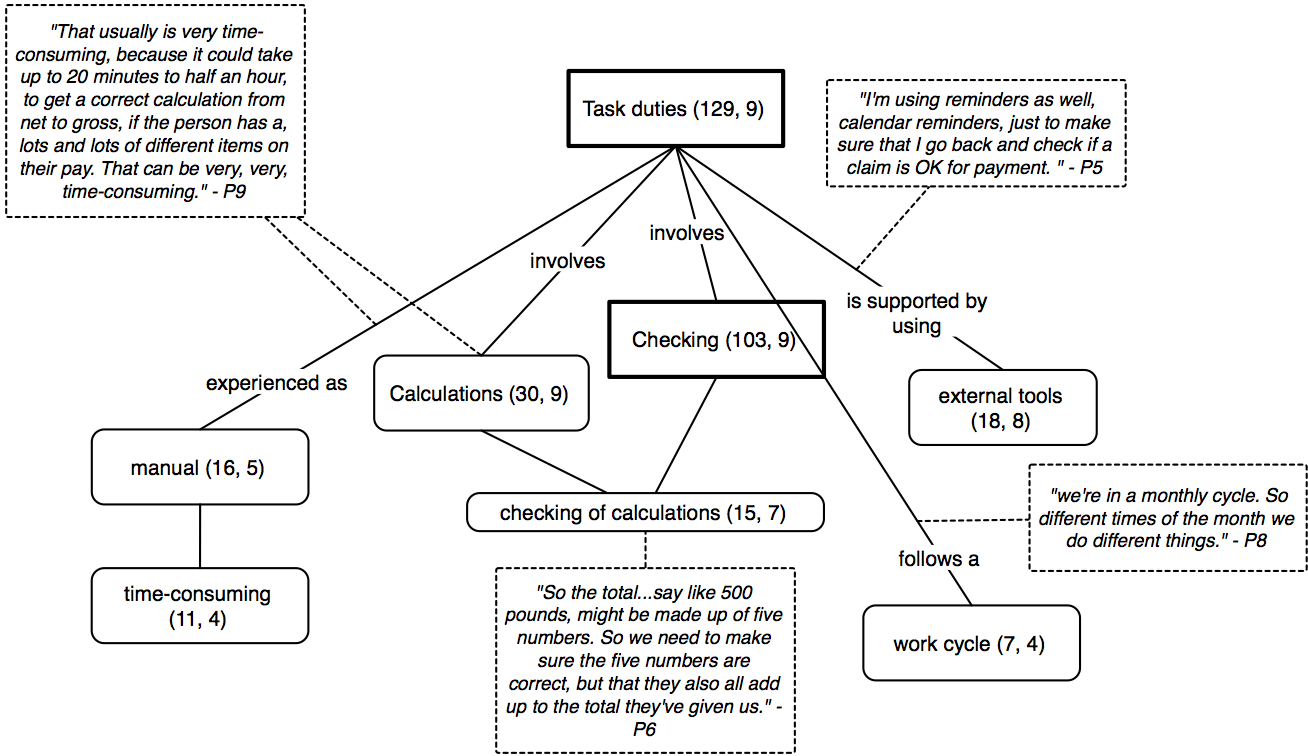
\includegraphics[width=\textwidth]{images/Study1/Task.png}
\caption[Study 1 Task diagram]{Diagram showing the theme Task. The numbers in parentheses indicate the number of quotes and the number of participants who mentioned it, respectively.}
\vspace{-9pt}
\label{fig:ch3_task}
\end{figure}
A common data entry task was entering expenses. Interviewees received expense claims from students and staff and had to check the information was correct. They then had to enter this data, along with other information such as budgetting and staff information, into a computer system.
All interviewees mentioned a large part of their job was checking that data was correct. In addition to transcribing and checking individual numbers, participants also mentioned they often have to perform and check calculations.
 Some tasks, such as calculations, had to be done manually and this was described as time-consuming. People used several external tools in their environment to support them in their tasks. For instance, P7 and P8 had paper sheets on their desk with information they frequently had to look up, so they could easily use this to check if the input they had received was correct.

Some people worked according to a work cycle, which meant they did different things at different times of the month. One week could be reserved for checking all the data they received from another department, while another week could be spent on solely inputting data. 

The time spent on each task differed: checking data on a short expenses form could be completed in two minutes, while a single calculation could take between 20 and 30 minutes. Two participants experienced dealing with a lot of data entry as tiresome.

\newpage

\subsubsection{Checking}\label{subsec:Checking}
\begin{figure}[!ht]
\centering
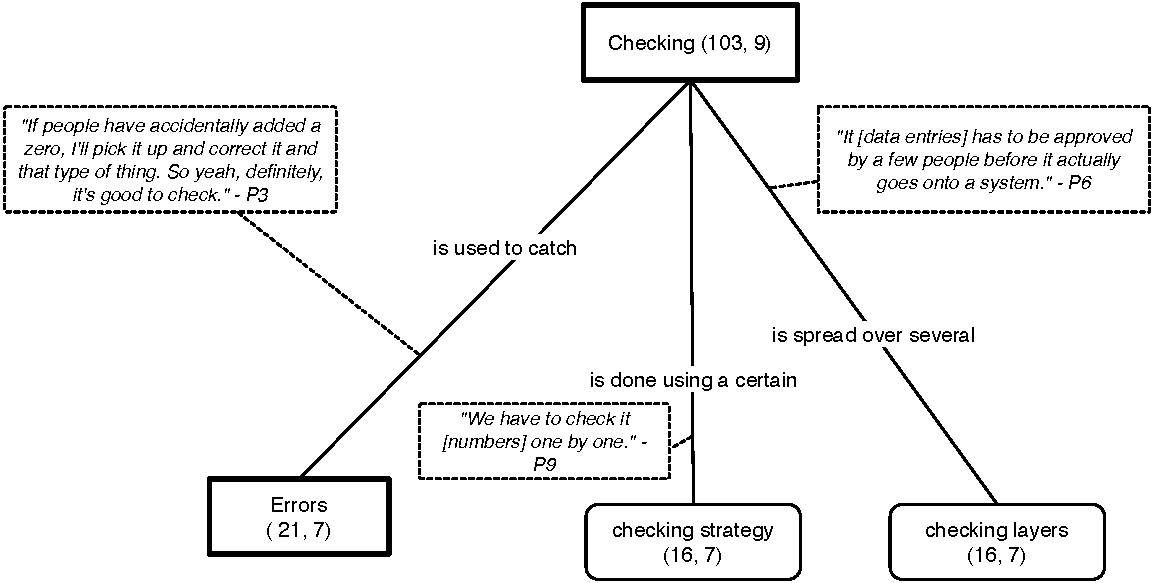
\includegraphics[width=\textwidth]{images/Study1/Checking.pdf}
\caption[Study 1 Checking diagram]{Diagram showing the theme Checking.}
\vspace{-9pt}
\label{fig:ch3_checking}
\end{figure}

All participants talked about checking data input for errors as a part of their job. Data was checked by several different people and departments before it was submitted. People's experience with this checking system differed: P3 felt that an error would be caught eventually because it goes through so many different layers, whereas P9 said it made people less careful about making errors and therefore they often received erroneous data. Sending wrong input back slowed the process down, and P8, who acted as the last person in his department to check before it gets submitted, warned that even with extra human checks not all errors get caught. 

People had to both check their own data input, as well as double-check other people's input. They maintained different checking strategies, ranging from checking each data item one by one to entering a group of data items first and then checking. 


\begin{table}[htp]
\centering
    \begin{tabular}{ | l | p{10cm} |}
    \hline
     \textbf{Participant} & \textbf{Quote} \\ \hline
    P3 & \textit{"we try and pick it [errors] up and then obviously there's all the different stages that pick it up as you go along."}\\ \hline
    P9 & \textit{"the departments actually sometimes treat us as a checking system [laughs], but they shouldn't really, the schools. Because we're here just to make sure that people get paid correctly. But even though we are like a second check, we feel sometimes that we are the first checkpoint."} \\ \hline
    P7 & \textit{"All this piece of work, when we input in the system, will be actually checked by another person... my manager will print it out, and then check... other colleagues will double-check it for you as well, the calculations."} \\ \hline
    P8 & \textit{"one of these errors could be things that are missed during the checking."} \\ \hline

    \hline
    \end{tabular}
    \caption[Study 1 checking quotes]{Verbatim quotes taken from the interview transcripts that were about checking.}
    \label{table:ch3_checkingquotes}
\end{table}%

\begin{table}[htp]
\centering
    \begin{tabular}{ | l | p{10cm} |}
    \hline
     \textbf{Participant} & \textbf{Quote/note} \\ \hline
    P1 &  first puts in all the details, then when done checks everything against the source. \\ \hline
    P7 & when entering numbers from paper to computer, mostly looked at paper form and the number pad; only looked at screen after finishing entering all the numbers from the form to check. \\ \hline
    P5 & \textit{"We would go by the receipt, so we would try to make sure that the receipts are in order."} \\ \hline

    \hline
    \end{tabular}
    \caption[Study 1 checking own input]{Checking own input when entering data.}
    \label{table:ch3_owninputquotes}
\end{table}%

\begin{table}[htp]
\centering
    \begin{tabular}{ | l | p{10cm} |}
    \hline
     \textbf{Participant} & \textbf{Quote} \\ \hline
    P5 &  \textit{"The numbers on the expense form will be checked individually. So the total will obviously be, say like 500 pounds, might be made up of five numbers. So we need to make sure the five numbers are correct, but that they also all add up to the total they've given us."} \\ \hline
    P6 & \textit{"The numbers on the expense form will be checked individually."}\\ \hline
    P9 & \textit{"We have to check it one by one."} \\ \hline

    \hline
    \end{tabular}
    \caption[Study 1 checking other people's input]{Checking other people's input.}
    \label{table:ch3_otherinputquotes}
\end{table}%

\clearpage
\subsubsection{System}
\begin{figure}[!ht]
\centering
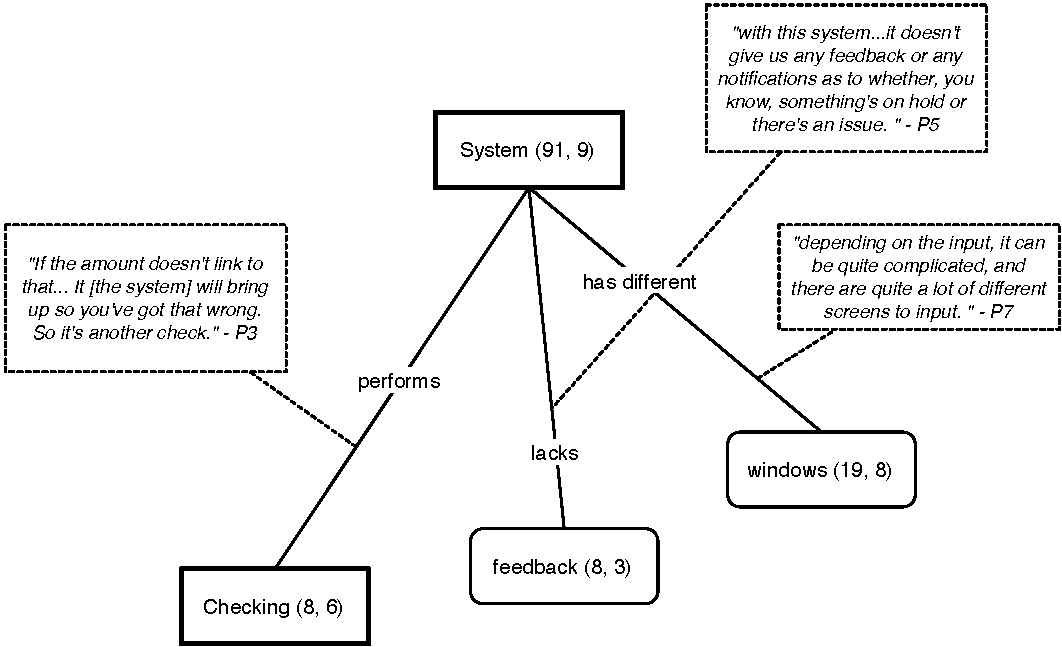
\includegraphics[width=\textwidth]{images/Study1/System.pdf}
\caption[Study 1 System diagram]{Diagram showing the theme System.}
\vspace{-9pt}
\label{fig:ch3_system}
\end{figure}

Data had to be entered into an information system on a computer. Some participants mentioned the system was another way to check for erroneous data entries: if the allowed number range of a variable was known, the system would let the user know if an out-of-range number was entered. However, it was also mentioned that one issue with the financial data entry system was that it did not give feedback if there was an issue or error.

The information needed for one task was usually spread over several windows on the computer, so sometimes people had to flick back and forth or memorise certain information from one window to use in another window. 

\clearpage
\subsubsection{Environment}
\begin{figure}[!ht]
\centering
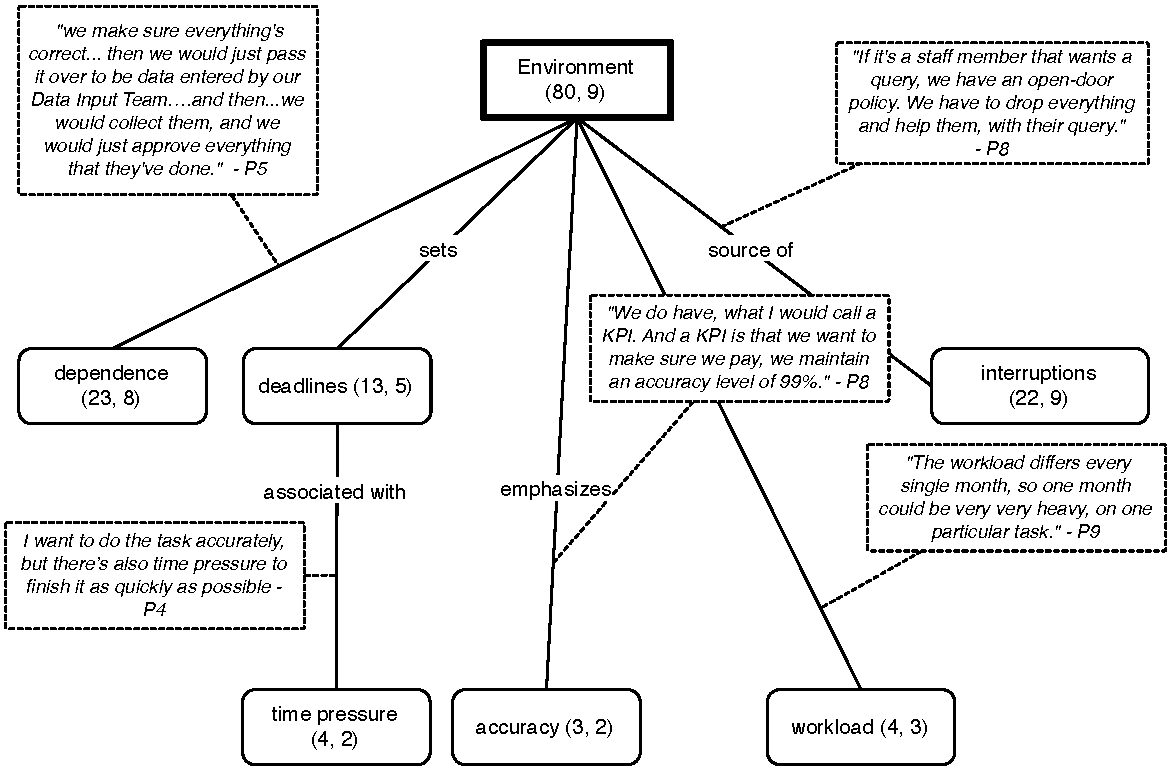
\includegraphics[width=\textwidth]{images/Study1/Environment.pdf}
\caption[Study 1 Environment diagram]{Diagram showing the theme Environment.}
\vspace{-9pt}
\label{fig:ch3_environment}
\end{figure}

Every time people described the environment they were working in, this was grouped under the Environment theme. The environment could be their immediate physical setting, or their organisation in general. 

All participants experienced interruptions during work. P8 mentioned he had to pause his task immediately if a staff member needed his help, but considered these interruptions part of his job. Other interviewees mentioned they tried to concentrate on the task at hand first, but did briefly attend to interruptions such as e-mail notifications, in case it was important.

People were dependent on other departments to finish a task. For instance, P5 checked paper expense forms, but did not enter these into the system herself. 

Some participants felt the pressure to be both accurate in data entry, as well as finish it quickly because of deadlines. The workload varied throughout the year.

\newpage
\subsubsection{Data}
\begin{figure}[!ht]
\centering
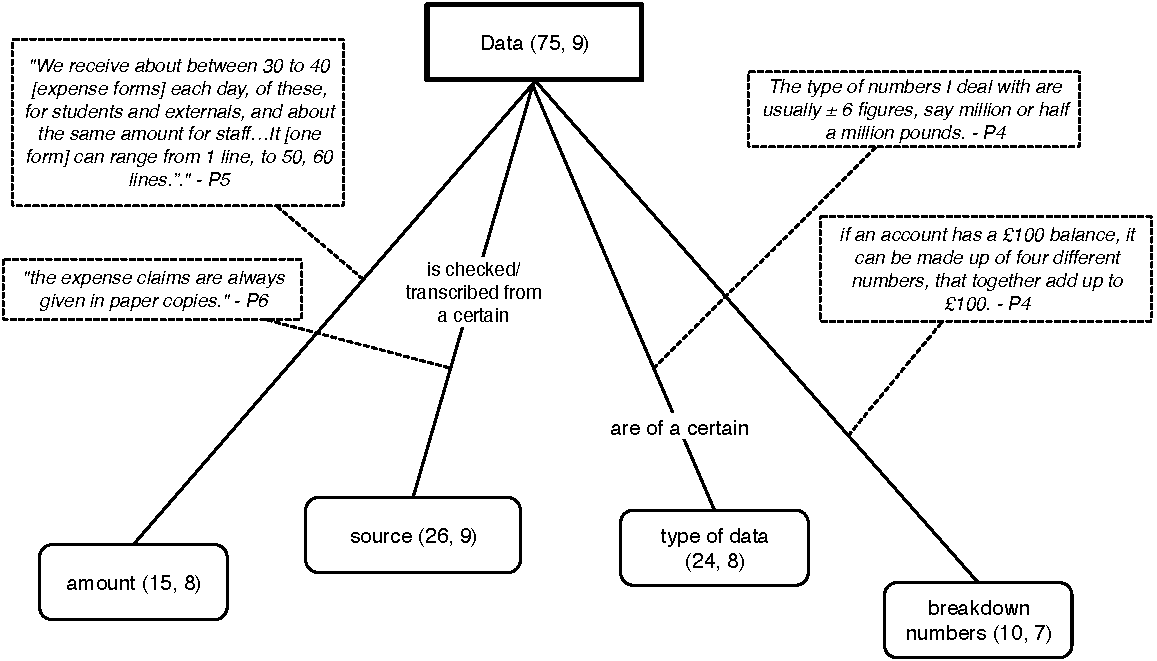
\includegraphics[width=\textwidth]{images/Study1/Data.pdf}
\caption[Study 1 Data diagram]{Diagram showing the theme Data.}
\vspace{-9pt}
\label{fig:ch3_data}
\end{figure}

Participants had to retrieve data from various sources. Some of the sources were electronic, such as Excel spreadsheets and Word documents. Some information had to be looked up in databases and work e-mails. Other information was received on paper sheets, and some participants had printed out information they frequently needed and had placed this on their desk. People had to transcribe numbers from paper onto a computer system for at least a part of their tasks. Some people worked with two screens.
The amount of data that people dealt with differed. P5 said that for expenses alone, the amount of numbers she received each day to check and input ranges from 100 to 6000 numbers.
People primarily dealt with numeric data, such as financial data and IDs. The monetary numbers they dealt with ranged from five to millions of pounds. Participants also entered and checked alphanumeric and non-numeric data such as employee names, addresses and bank account details.

Numeric data consisted of individual numbers, as well as groups of numbers that together made up a new number, such as the total amount of money spent on a project. Participants had to both check and transcribe each individual number, and check that the calculation was correct. 

\ \clearpage

\subsubsection{Errors}
\begin{figure}[!ht]
\centering
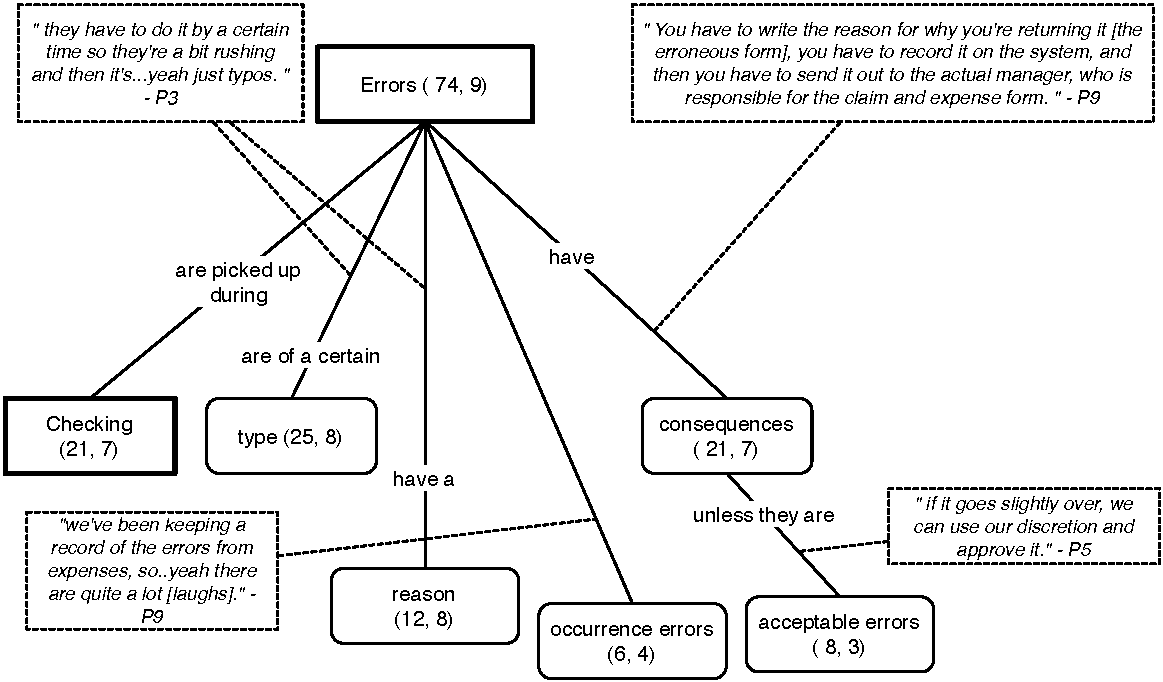
\includegraphics[width=\textwidth]{images/Study1/Errors.pdf}
\caption[Study 1 Errors diagram]{Diagram showing the theme Errors.}
\vspace{-9pt}
\label{fig:ch3_errors}
\end{figure}

Participants discussed that errors happened frequently, and talked about errors they spotted from other people. Visual checking was mentioned as the main method to catch and correct errors in time, but when possible the computer system sometimes checked for erroneous data as well. Errors that were made were typos, miscalculations, or people had the wrong information to enter. For instance, P7 mentioned that when salary rates change, employees often keep entering their old salary rate on claim forms, which then has to be corrected. The main explanation people gave for errors was that it is human to make mistakes, but it was also mentioned people are under time pressure, and that people rely on the fact it will be checked by another person, which makes them less careful in entering accurate data. 
If an error was spotted, this had certain consequences depending on if the error was acceptable or not. If the error was sufficiently small, it could be either processed or corrected without negotiation, but if it was a large error, it had to be sent back or forwarded to a higher authority for approval. 

P1 highlighted project IDs used to be letters but are now numbers, which are harder to memorise, and he felt it was easier to make a mistake. P4 worked with both paper and digital files to transcribe data from, but preferred digital files because he felt it was much easier to make an error and omit figures when transcribing from paper.

\begin{table}[htp]
\centering
    \begin{tabular}{ | l | p{10cm} |}
    \hline
     \textbf{Participant} & \textbf{Quote/note} \\ \hline
    P6 &  \textit{"it's quite common that we have to return an expense or payment back to someone. It happens quite often, yeah."} \\ \hline
    P4 & Yes all the time, lots of typos.\\ 
    \hline
    \end{tabular}
    \caption[Study 1 errors quotes]{People mentioned errors occur quite frequently.}
    \label{table:ch3_occurrenceerrorsquotes}
\end{table}%


\begin{table}[htp]
\centering
    \begin{tabular}{ | l | p{10cm} |}
    \hline
     \textbf{Participant} & \textbf{Quote} \\ \hline
    P3 &  \textit{"sometimes it's because people have done typos, done too many zeroes, or left out a zero."} \\ \hline
    P5 & \textit{"the expense breakdown doesn't match what (...) whatever they put as the grand total."}\\ 
    \hline
    \end{tabular}
    \caption[Study 1 type of errors quotes]{The type of errors.}
    \label{table:ch3_typeoferrorsquotes}
\end{table}%


\begin{table}[htp]
\centering
    \begin{tabular}{ | l | p{10cm} |}
    \hline
     \textbf{Participant} & \textbf{Quote} \\ \hline
    P9 &  \textit{"Because the departments actually sometimes treat us as a checking system [laughs], but they shouldn't really."} \\ \hline
    P7 & \textit{"Yeah, human laziness or something [laughs]."}\\ \hline
    P8 & \textit{"sometimes, you know, through human error, you know, things don't get paid properly."} \\
    \hline
    \end{tabular}
    \caption[Study 1 reasons for errors quotes]{The reasons for errors.}
    \label{table:ch3_errorreasonsquotes}
\end{table}%


\begin{table}[htp]
\centering
    \begin{tabular}{ | l | p{10cm} |}
    \hline
     \textbf{Participant} & \textbf{Quote/note} \\ \hline
    P5 &  \textit{"generally we tend, we try not to send claims back to departments because they might get lost in the post, and it's an inconvenience as well. So we try to... resolve it ourselves.."} \\ \hline
    P4 & We allow a certain amount of tolerance; if it turns out the thing you bought has actually decreased value and is now  \pounds40, we will allow to return  \pounds50\\ \hline
    P7 & \textit{"we normally e-mail the budget holder to say... what you authorised is actually different. But for this kind of thing, it's only 10 pounds...we normally just process this without contacting them."} \\ \hline

    \hline
    \end{tabular}
    \caption[Study 1 acceptable errors quotes]{Acceptable errors.}
    \label{table:ch3_acceptableerrorsquotes}
\end{table}%

\clearpage
\subsubsection{Strategy}
\begin{figure}[!ht]
\centering
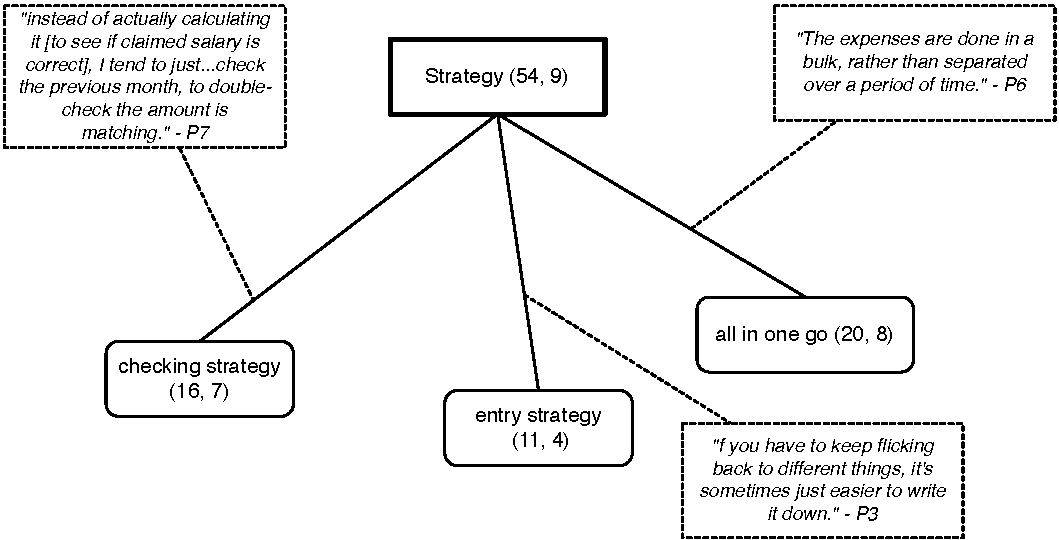
\includegraphics[width=\textwidth]{images/Study1/Strategy.pdf}
\caption[Study 1 Strategy diagram]{Diagram showing the theme Strategy.}
\vspace{-9pt}
\label{fig:ch3_strategy}
\end{figure}

Eight of nine interviewees saved up data to enter it all in one sequence. If they received forms with data input to check or enter, they saved these for later and then processed all the forms. P1 indicated he processed forms in batches of at least five forms, and found it disruptive to do just one or two and then switch to something else. 

P2 was the only interviewee that processed forms with numbers to enter as they came in, but did admit that if she had more data to fill in, she would probably do it in a more efficient way.

Some people said they preferred batching their work so that they entered all data into a single system at once because it is quicker and easier to do the same type of tasks in one sequence, and when that is finished concentrate on another task. P4 mentioned he does them all at once because he gets the forms in a bulk and feels pressure by his boss to finish them all immediately, rather than spread them over time. P6 explained he postpones processing expense forms until the deadline to submit forms for that month has passed, after which he does all forms in one sequence. 

People also talked about other strategies they used to do their job more efficiently. For instance, if they had to get out of the system to look up information digitally and then get back to the system window to enter it, they preferred to memorise the information, rather than flick back and forth and look it up each time they needed it. With numbers they had to enter frequently such as project codes, they memorised it even if they did not deliberately choose to do so. If the information to remember was complicated, they would write it down.

As discussed at the \nameref{subsec:Checking} section, people had different checking strategies and the number of times they looked back to the data source to check it against the data input varied. P7 said she sometimes deals with similar calculations, so she prefers to check the calculation she did last time rather than calculate it again. 

People explained that a lot of numbers they enter are calculated from other numbers. Some people liked to write out and keep a record of their calculation, in case someone had any questions on how that number was calculated.

\begin{table}[htp]
\centering
    \begin{tabular}{ | l | p{10cm} |}
    \hline
     \textbf{Participant} & \textbf{Quote/note} \\ \hline
    P3 &  \textit{"I just try and do it in the quickest way...It's nice, once you've done it, it's completed, so it's sort your weight lifted [laughs]. So you don't need to think about it again."} \\ \hline
    P6 & \textit{"the expenses are done in a bulk, rather than separated over a period of time. When I'm doing it lots at a time, I think once you get into sort of the hang of it, it gets done a lot quicker than..you just get used to putting them in, and inputting it all."} \\ \hline
    P9 & \textit{"I try to concentrate on my task...I try to do one task [i.e. doing all expenses], finish one, and then do another."} \\ \hline
    P4 &  It's difficult to take rests or even switch in-between number entry tasks because of the work pressure, and feels pressure by boss. \\ 
    \hline
    \end{tabular}
    \caption[Study 1 batching quotes]{Most participants entered all numbers in one go.}
    \label{table:ch3_inonegoquotes}
\end{table}%

\begin{table}[htp]
\centering
    \begin{tabular}{ | l | p{10cm} |}
    \hline
     \textbf{Participant} & \textbf{Quote/note} \\ \hline
    P3 &  \textit{" I wouldn't necessarily have to [memorise numbers], It's more just if you have to keep flicking back to different things, it's sometimes just easier to write it down, or just try and remember it. But you can obviously take the long version and keep flicking back to the correct screen."} \\ \hline
    P2 & \textit{"we have different grants and different project codes as a result, but you, because you use them so much, you end up remembering them."} \\ \hline
    \end{tabular}
    \caption[Study 1 strategy quotes]{Examples of strategies people used.}
    \label{table:ch3_strategiesquotes}
\end{table}%

\ \clearpage

\subsubsection{Importance of accuracy and paper trails}
\begin{figure}[!ht]
\centering
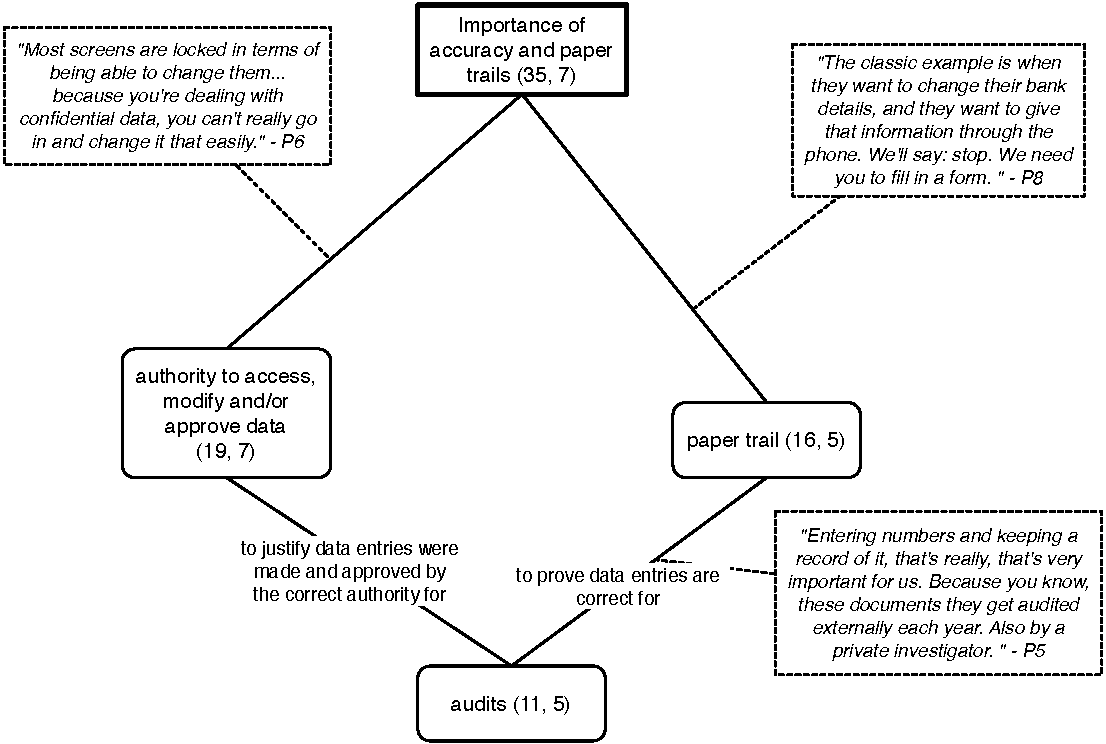
\includegraphics[width=\textwidth]{images/Study1/Papertrail.pdf}
\caption[Study 1 Importance of accuracy and paper trails diagram]{Diagram showing the theme 'Importance of accuracy and paper trails'.}
\vspace{-9pt}
\label{fig:ch3_papertrail}
\end{figure}

Because interviewees were working with sensitive financial data, another theme was importance of accuracy and paper trails.
Some data could only be entered in the system and modified by certain people.
Large figures had to be approved by a superior first before it could be processed, so it was clear to an auditor that expenses were made with the correct approval.
Hard copies of data had to be archived and were checked by external auditors. For instance, all expenses were claimed on paper forms, and had to have the original receipts as evidence that the expense claims were correct. Some data could not be given over the phone but had to be written down and sent via a paper form.

\pagebreak

\subsubsection{Other}
\begin{figure}[!ht]
\centering
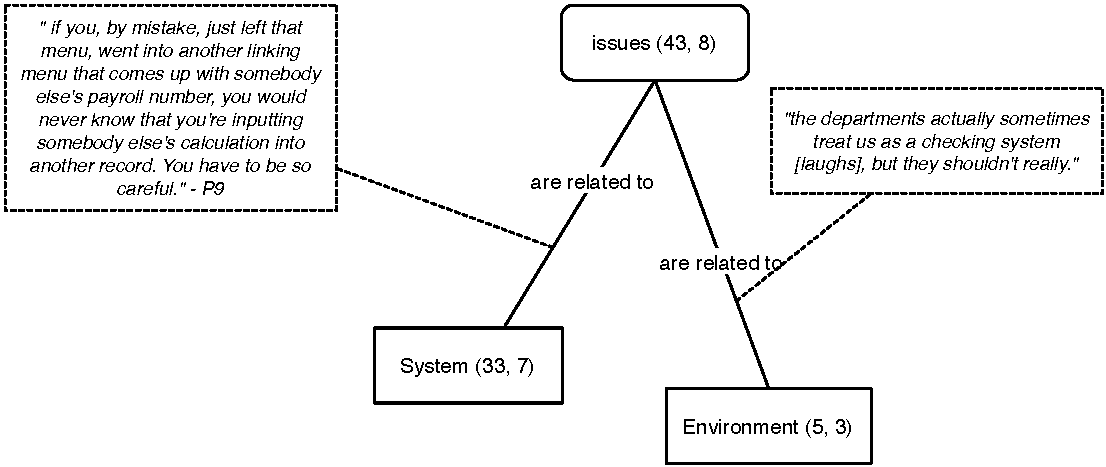
\includegraphics[width=\textwidth]{images/Study1/Other.pdf}
\caption[Study 1 Other diagram]{If people described issues, it usually had to do with the system.}
\vspace{-9pt}
\label{fig:ch3_other}
\end{figure}

Interviewees mentioned several issues they experienced. Most of the time, the issues had to do with the current data entry system they were using. P7 mentioned number entries on the computer screen were small and hard to read, and could not be enlarged. P5 mentioned she did not get notifications from the system if there was an issue with a payment, so she would not know about it until staff members would call up to complain they had not been paid yet.  Other issues had to do with the organisation, such as the experience that the multiple checking layers made people rely on other people to check their input.

\begin{table}[htp]
\centering
    \begin{tabular}{ | l | p{10cm} |}
    \hline
     \textbf{Participant} & \textbf{Quote/note} \\ \hline
    P5 &  \textit{"There are other issues. You could say I think hundreds, I mean not just with the work that we do on expenses, but across [university A], across [university A] Finance, the Finance division...We just have to kind of work our way around the system and you know, adapt to it."} \\ \hline
    P7 & \textit{"It's only the matter of how you get used to the Payroll system. Because companies have different systems, the data inputting can take a while to get used to it."} \\ \hline
    P9 &  \textit{"You know, all systems are a bit funny, I think. But you just gotta get used to it."} \\ \hline
    \end{tabular}
    \caption[Study 1 issues quotes]{Issues that participants experienced with the system.}
    \label{table:ch3_otherquotes}
\end{table}%

\pagebreak

\subsection{Discussion}
The purpose of this study was to gain a better understanding of the type of data entry tasks in financial offices, and the physical environment in which these are conducted. For this purpose nine interviews were conducted with staff from two public universities who worked with financial data. The main findings of the study are: 

\begin{itemize}
\item 
people have to get the data to enter from various sources, with varying information access costs
\item 
people batch their work to enter a lot of data entry at once, and minimise switching between tasks. 
\item 
data entry errors are common, and the current solution is to have data entered and checked by multiple people before it gets submitted to the system
\end{itemize}

\subsubsection{Information sources and access costs}
A prevalent data entry task of participants' work was processing expense claims from university staff and students. A substantial part of this task is not just entering the data but also collecting it from multiple sources. For example, the expenses had to be entered from paper forms and receipts, foreign currencies had to be converted and copied from a website, and staff and financial information had to be retrieved from sources such as electronic spreadsheets, databases and e-mails. 
In data entry experiments, the data is often shown on a computer, to make it easy to manipulate. This was sometimes the case in the office setting studied here, but data was also transcribed from paper sheets into a computer. Furthermore, in lab experiments people are often only presented with the data they have to enter and sometimes are given only one data item at a time. The sources from which people had to enter data in this study usually contained a lot of data, not all of which was relevant to the task. The amount of irrelevant data on the sources can increase the time people need to look up the information they need.

The cost to access the information sources differed. For instance, some paper sheets were on people's desk, but some paper sheets had to be retrieved elsewhere. Sometimes participants had to go through a large spreadsheet, before they found the number they needed to copy. Participants also dealt with multiple windows on their computer screen, and sometimes needed to switch between different windows. Instead of flicking back and forth to view information they had to enter in another window, people said they preferred to memorise it. This supports previous research which showed that people make strategic use of internal and external resources and do not always maximise off-loading cognition to external resources \citep{Gray2006}. Even though participants were aware they did not have to remember information, they found this easier and faster rather than looking it up or writing it down. 

This strategy allows people to be faster, but carries the risk that they misremember it. In previous studies, trying to hold more items in memory during a copying task increased errors \citep[e.g.][]{Morgan2009}. However, in these studies people had to copy over coloured blocks, which were abstract to the participants and may have been too hard for participants to memorise \citep{Waldron2011}. In the current study, the information had some meaning to the users, and even if they were dealing with abstract information, such as project codes or ID numbers, some items were entered more often than others. Participants mentioned that even if they did not make a conscious effort to memorise these, they had to enter these numbers so often that they ended up remembering them. This is in line with prior findings that some numbers are more familiar than others, and that these familiar numbers are more strongly represented in memory \citep{Wiseman2014}. 

If information to copy is familiar and contains numbers and text, making the effort to encode the information more deeply has been shown to make people more accurate \citep{Gray2004, Soboczenski2013}. It is therefore not clear if the effect of a memory-based strategy on accuracy, as found in \citep{Morgan2009}, would extend to copying the material of this study.

People used some external tools to aid memory. For example, some participants had printed sheets with information they used and entered often, so they did not have to repeatedly look this up in the system. They also used calculators and pen and paper to perform calculations.

\subsubsection{Batching data entry tasks}
Eight of nine participants batched data entry tasks to do them all at once, rather than spread them over time. The only participant who processed expense forms as they came in said she did not receive a large amount of forms. She explained that if she dealt with a higher volume of expenses, she would probably do it in a more efficient way.

There were different reasons behind the strategy to enter a large amount of data in one sequence. One participant received forms in a bulk, and felt time pressure to finish them all at once, rather than spread them over time. The other seven participants said they received forms on an ad-hoc basis, but deliberately saved them until a specific moment and then processed them all in a bulk. They preferred to focus on one task at once, and some people stated that it made them faster in entering data after a while. 

This is consistent with Healy et al.'s \citeyearpar{Healy2004} study, where learning effects could be measured in a number entry task. However, in their experiment participants became faster but also more erroneous in entering data. In the current study, P3 mentioned that most of the errors she picks up from colleagues are typos caused by rushing to finish the task. P4 mentioned that he wants to enter numbers accurately, but that there is a time pressure to finish things in time. This is in line with the speed-accuracy trade-off discussed in literature, and that a sense of urgency may cause people to enter numbers faster but at the expense of a higher error rate \citep{Lin2011, Lin2013}.
\citet{Healy2004} recommended regular breaks when entering large amounts of data to maintain accuracy, but P4 in the current study explained it is difficult to initiate breaks himself, when he feels a time pressure to finish it.

\subsubsection{Multiple checking stages}
In order to prevent errors, input was entered and checked by multiple people before it was allowed to be submitted into the system. This checking method is similar to \citeauthor{Reason1990}'s \citeyearpar{Reason1990}  Swiss Cheese model, where multiple checking layers are used to minimise the risk of errors. However, as a result of this people seemed less careful in checking their own input, because they knew it would be checked by someone else. 

In previous studies, providing incentives for people and introducing lockouts into the data entry interface has been shown to influence how carefully people check their input \citep{Li2015, Gould2015}. The findings from the current study suggest that how and whether people check also partly depends on what the primary objective of their task is: entering or checking input.

When people were asked to check other people's data input, they checked each data item one by one. However, when they had to enter data themselves, they tended to chunk data items and only checked their entries when they had entered all items on one source. This finding is based on both observations when participants demonstrated a number entry task, as well as descriptions people gave on how they tend to perform their task. When people are asked to enter data, checking their input is not the main focus of the task, but rather a post-completion step that has to be performed after the main goal of entering data has been completed. It is well known post-completion steps are prone to errors, as it is not part of the main goal of the task \citep[e.g.][]{Byrne1995, Li2006, Li2008}.

It could also be that people were aware their input was going to be checked by another person, and therefore did not spend as much effort trying to check it properly. When talking about checking other people's input, people emphasised how it was important that each data item was checked carefully. However, when they talked about their own input, they tended to emphasise this less and mentioned another person would double-check it anyway.

\subsubsection{Summary}
The purpose of this study was to get a better understanding of data entry tasks associated with finance administration office work, and the context in which these tasks are done. While it was informed by previous data entry research, it did not have a particular theoretical framework prior to undertaking the study to inform and guide the data collection and analysis. 

A prevalent data entry task of the participants was processing expense claims from university staff and students. A substantial part of this task was not just entering the data, but also collecting it from multiple sources with varying information access costs. As my data collection and analysis progressed, it emerged that framing the findings in terms of different information access costs (IAC) of these information sources had the potential to provide a useful lens on the data for informing the design and evaluation of data entry systems. As the study looked at the wider context of participants' data entry work and did not focus on entering expenses per se, it was not recorded which sources people needed and how they looked up information.

The aim of the next study is to investigate the information sources people need for an expenses task, and how they currently manage subtasks of looking up information from an expenses task. 
%Sometimes the cost to access an information source was low, and people could easily access it and look at it while entering it. Other times the cost was high, and people had to go back and forth between the window that showed the information, and the window in which they had to enter the information. Theory suggests that these different access costs have an impact on strategy, speed and accuracy. In previous experimental studies, an increase in IAC made people check the information source less and instead enter what was in their head. This can make people more efficient as it minimises switching between the information source and the input interface, but if the information in the head is wrong, it increases errors. In these previous studies, it increased errors, but the studies made use of abstract artificial information, which may have been too hard for participants to memorise. 
%In the current study, people had to copy numbers and text. Previous studies showed that when looking at text and/or numbers, a deeper encoding of the information in memory makes people more accurate in entering the information. 
%The next study aims to see if the effect of IAC on a copying task extends to copying numbers, which people have experience with copying and can more easily memorise.

\section{Study 2: Information sources for entering expenses}

\subsection{Introduction}
%The purpose of Study 1 was to get a better understanding of data entry tasks associated with finance administration office work, and the problems employees currently experience carrying out these tasks. I did not use a particular theoretical framework prior to undertaking the study to inform and guide the data collection, and did not explicitly focus on the different information sources needed for entering expenses per se.  It was only as data collection and analysis progressed, that it emerged that framing the findings in terms of different IACs had the potential to provide a useful lens on the data for understanding people's data entry strategies, and informing the design and evaluation of the data entry expense systems.

%A prevalent data entry task in the financial offices observed in Study 1 was entering expenses. For this task, workers had to look up information from multiple sources, and the IAC for each source differed. Study 2 showed that when people have to copy data from one source in a lab setting, and the IAC of this source increases, they try to memorise more information in order to reduce visits to the source. In the experiment, all information came from one source and was the same type, i.e. either all items were numbers, or all items were colours. For each participant, the IAC was the same throughout the experiment: it was either low, medium, or high. 
A common data entry task observed in Study 1 was entering expenses. Office workers receive expense claims from staff, check the information is correct, and enter it, along with other information, into a computer system. They have to enter different types of information such as numbers and alphanumeric strings, these do not all come from the same source, and different sources can have different IACs. For example, some information can be recalled from memory, some has to be typed from a paper sheet, some numbers have to be calculated first, and some information has to be looked up in an electronic information system. 

The purpose of this study is to investigate the information sources people need for an expenses task, and how they currently manage subtasks of looking up information from an expenses task. Do they look up information as they need it, or get all the required information first and then enter it? They may also change their strategies as they get more experienced with the task and know where to get the information from, or enter all information that is easy to access first.

Ten finance employees will be observed at their workplace, with a particular focus on the information resources they need and use for entering expense claims into the financial computer system. I will shadow them doing their work, and will ask them to demonstrate the task while thinking aloud. They will be interviewed afterwards  and I will ask them questions about observations I made. 

In order to better understand how people switch between applications for office work, \citet{Cangiano2009} made screen recordings of workers' activities in a law office. They then played these back to the workers, and asked them to explain their activities. These screen recordings were useful for workers to accurately recall what they were doing at the captured moments, and why they had certain windows open. 

One of the advantages of using screen recordings is that it provides a detailed account of activity, however there are also privacy issues and not all participants agree their activity to be recorded \citep{Rule2015}. In a finance setting, there are additional confidentiality issues and participants may not be allowed to share financial data. Participants in the current study will instead be video recorded while doing the expenses task. The video recordings capture the participants' interactions with the artefacts involved in the task, but the financial data on the information sources cannot be identified from these recordings. The video recordings will be used to supplement my written observation notes, and after the observation part of the study, some video segments may get played back to participants and they will be asked to explain what they were doing at certain moments.

\subsection{Method}
\subsubsection{Participants}
Ten participants will take part in the study. They will be employees from financial offices at public universities dealing with processing expense claims. A combination of convenience and snowball sampling will be used to recruit the participants. Convenience sampling will be applied by distributing flyers, sending invitations to opt-in mailing lists of Finance departments from several universities, and by asking people from the user group that are familiar to the researcher. In addition, snowball sampling will be used by asking participants if they know colleagues who would potentially be interested to participate in the study. 
Ideally a range of experience levels will be included, from beginner to experienced level. Participants will be reimbursed with \pounds15 and be entered in a prize draw to win \pounds50. 

\subsubsection{Contextual inquiry}
My data collection will be informed by using the methodological approach of contextual inquiry.
Contextual inquiry is a combination of observation and interviewing users and their everyday work, with the aim to use the findings to inform design of the systems they use \citep{Beyer1998}.
\citet{Beyer1998} argue that observing participants carrying out their work can reveal concrete details, and it can help participants to recall past situations of carrying out work. It is therefore considered to be an appropriate method for the aims of this thesis, as it involves understanding users' expenses work with the aim to translate it into design implications for their expenses system. 

I will follow the four stages of \citet{Beyer1998}:
\begin{enumerate}
\item 
Interview

In this part, the participant will typically be asked general questions about their work. This part is primarily to make the participant feel comfortable and start the conversation easy. As I have already gained an insight on finance employees' general work in Study 1, this interview will be more particularly focused on their expenses task. Participants will be asked about their experience with the system  and the resources they use, to get an idea of what they consider resources.
\item 
Transition

In this part, the participant will demonstrate the expenses task and will be asked to think out loud. I will prompt questions if the participants falls quiet or will ask to elaborate if something interesting or unusual happens.
\item 
Observation

In this part, the participant will do his/her work while I observe and make notes. If allowed, participants will be video recorded. The participant will go about doing work without explaining what he/she is doing and why. 
\item 
Summary

In the final stage, I will ask questions about observations I made. I will summarise to the participant what I have found and check if this is correct. If some parts of the observation need clarification, segments of the video recording may get played back to participants, and they will be asked to explain what they were doing at certain moments.
The participant will be thanked and debriefed.
\end{enumerate}

\subsubsection{Materials}
Materials that will be used during the contextual inquiry are a voice recorder, a video camera, an interview script with guiding questions, a checklist to guide the observation and think-aloud part, a notebook and pen to make notes, and a consent form and information sheet for the participant.
A number of interview questions will be written out beforehand. These questions are used as a starting point to get the participant talking and guide the interview. Based on what the participant is saying follow-up questions will be asked. 

\subsubsection{Pilot study}
In order to test the suitability of the study set-up, a pilot study was conducted with a financial administrator at a university who dealt with processing expenses. The study took place at the university, and notes were taken with pen and paper. 

Initially, the intended method of this study was to conduct a contextual inquiry, followed by a week-long diary study where office workers would log diary entries of their expenses tasks. The aim of this diary study would be to get a further insight in additional information sources they may sometimes use, that were not covered in the contextual inquiry.  Participants would submit a diary entry either by writing down a description or by taking a photograph of the task setting, showing the information sources. At the end of the day, they would have to answer the following questions about their short entries: what information did you need, where did you need to get it from, and when did you look up the information. This method built on a study by \citet{Sohn2008}, where participants kept a diary of their mobile information needs and how they addressed those needs. 

The administrator explained that expense tasks usually are conducted in the same manner, and predicted I was unlikely to find a lot of instances that differ from my observations of having office workers do the task.
Furthermore, by observing them I am able to see the access people have to the resources and how much time it takes them to get the data, as well as when in the task they decide to look up information. This information would be more difficult to get insight to through diary entries.

It was therefore decided after this study to not conduct a diary study but instead only observe office workers, and ask them to explain their work.

\subsubsection{Ethical considerations}
The study has ethical approval from the UCL Research Ethics Committee [Project ID Number UCLIC/1415/001/Staff Brumby/Borghouts]. 

The advertisement will include what participants will be asked to do and what their reimbursement will be. 
Participants will be briefed at the beginning of the study. They are then asked to read and sign a consent form, and are given an information sheet with the study information and my contact details for them to keep. 
It will be explained they are free to withdraw from the study at any time, and that their data will be used for research purposes only. They will be asked for permission to audio record the interview, and video record them doing their work. It will be explained that the purpose of the study is to get a better understanding of how they normally go about their work with an aim to improve the system, and that there are no right or wrong ways of doing tasks. 

It will be explained that the purpose of data collection through photographs, screenshots, audio and video recordings  is to get an understanding of the information sources and interactions involved in an expenses task. Prior to the video part of the study, participants will review the setup of the video camera to confirm the camera is set up appropriately and does not capture any confidential data.

Participants will be informed that the data will be used for research purposes only and stored in accordance with the Data Protection Act 1998. Their data will be anonymised and when used in a report or academic paper, their data will not be directly identifiable. Names of participants or the organisations they are working at will not be included in the interview notes and transcripts.

\subsection{Data collection and analysis}
The sessions will be audio recorded, and the interviews and think-aloud verbal protocols will be transcribed verbatim. I will take written notes during the think-aloud and observation parts of the study. The transcripts and notes will be analysed using thematic analysis. The data analysis program Atlas.ti will be used to code the data. 

The think-aloud and the observation part of the study will be video recorded. The video recordings will be used to complement my notes taken during observation. Furthermore, some segments will get played back to participants at the final stage of the study and they will be asked to explain what they were doing at certain moments.

The video recordings will be used to identify information sources involved in the expenses task, and the frequency and timing of visits to each information source during the task.

Screenshots and photographs of the information sources will be collected.

\subsubsection{Expected findings}
\begin{itemize}
\item
People will have to switch multiple times between different data sources as part of the same expenses task.
\item
The IAC of these data sources varies. 
\item
If IAC of an information source is high, people will rely more on knowledge in the head: they will copy over more data in one go when IAC is high.
\item
Batching is a task planning strategy that gets employed by people with some experience in the task, in order to reduce switching between data entry tasks, and other tasks.  People will save up data entry tasks to do them all in one sequence.

Depending on people's experience and awareness of how costly it is to access information, people may plan their expenses task to reduce switching between entering and looking up information. They choose to enter all the low-IAC items first, in a batch, and then the high-IAC items second, also in a batch, rather than looking up each item as they need it.  An explanation for this is that they minimise the start-up costs of the entry task.

\end{itemize}
\subsubsection{Contribution}
\begin{itemize}
\item
Evidence that an expenses task is fragmented: people often have to go in and out of the expenses system to look up information.    
\item
Evidence that the IAC of the required information sources for an expenses task varies. 
\item
Evidence that depending on people's experience and awareness of how costly it is to access information, they will try to minimise switching between tasks.
\end{itemize}

\chapter{Understanding the effect of IAC on looking up information}

\begin{mynote}
\subsubsection{Chapter outline}
The previous chapter demonstrated that for an expenses task, people have to copy data from multiple sources that differ in terms of their IAC. This chapter describes two studies that explore the extent to which IACs influence strategies, speed and accuracy. 

Study 3 tests how IAC affects switching behaviour when copying from one source. It tested whether the effect of IAC on copying colours, as shown in previous studies, extends to copying numbers. Study 4 tests how IAC affects switching behaviour when information for one entry task has to be collected from multiple sources.
Together these studies intend to show that IAC affects how people switch between entering and looking up information.

\end{mynote}

 
\section{Study 3: Copying numbers from one source}\label{ch:Study2}
\subsection{Introduction}
Study 1 and 2 illustrated that people had to retrieve and copy data from multiple sources with varying information access costs (IAC). People were not always able to look at the data source while entering data, and information sometimes had to be briefly kept in memory before people could enter it.
In this situation, people have various options: they can decide to keep going back to the target source, reduce their memory load by writing it down, or keep as much of it in memory. Participants in Study 1 explained they tried to do it in the quickest way possible, and preferred to keep data in memory as this was often a faster strategy than writing it down, printing it out, or going back and forth between the source and the input window.

This is in line with previous lab studies, which showed that as the cost to access information increases, people increasingly rely on the information in their head rather than the information in the environment \citep[e.g.][]{Gray2006, Morgan2009}. People look at the target source longer before copying anything, but after one look, they do enter more items in one sequence before looking back. 

\citet{Gray2004} conducted a study where people had to copy over VCR programming information. Participants either had permanent access to the information, the information was covered by a grey box which could be uncovered by hovering over it with the cursor, or they were explicitly instructed and trained before the trial to memorise the information. The people in the latter condition were more accurate than the other conditions in entering the information. This shows that a deeper encoding of the information in memory makes people more accurate in entering the information. 

In later studies that further explored the effect of access costs on use of memory, the Blocks World Task (BWT) was used as a task paradigm, which requires people to copy a 3x3 grid of coloured blocks. In these studies, participants relied more on memory as the cost to access the target window increased. In one study, this memory-based strategy made participants better able to resume after interruptions by copying more blocks before having to revisit the target window \citep{Morgan2009}. Looking at overall task performance overall however, they did make more errors overall and took considerably longer to complete the task. In a later paper, the researchers reflected that the coloured blocks participants had to copy may have been too demanding to memorise \citep{Waldron2011}. This abstract visuo-spatial information did not bear any meaning to the participant, in contrast with the VCR programming information used in \citet{Gray2004} which is more familiar and easy to memorise. This suggests that the type of information to copy influences the effect that IAC might have on task performance, though the studies differed in task paradigm making it hard to compare their findings: in \citet{Gray2004} people were explicitly instructed to memorise the information and conducted a test prior to a trial during which they had to fill in the information, and could not continue until they had stated everything correctly. This ensured that people had the information well-memorised before they started the experimental trial. In the Blocks World Task studies, participants were not given this training or instruction.

Rather than training participants to memorise the information, \citet{Soboczenski2013} used an alternative approach to motivate people to encode the information more deeply. They conducted two studies where people had to transcribe text and numbers that were presented either in a black font colour or a harder-to-read grey font colour. Participants made fewer data transcription errors if data was shown in the harder-to-read font colour, both for transcribing text and numbers. In line with \citet{Gray2004}, these studies showed that when people do make the effort to more deeply encode information in a copying task, it can improve their accuracy.

In order to design data entry interfaces that support how people enter expenses from information sources with varying IACs, it is important to understand how these differences in IAC affect strategy and task performance. Relying on information in the head over information in the world can make it more likely for people to make errors in a copying task\citep{Morgan2009}, though other studies have shown that a deeper encoding of information can also improve accuracy if memorised well \citep{Gray2004, Soboczenski2013}. 

The study reported in this chapter replicates the BWT study, by using both coloured and numbered blocks.The purpose of this study is to see whether the effect on IAC on people's strategies and performance, as reported in previous BWT studies, holds when people have to copy numbers instead of colours.

It is expected that the effect of IAC on strategy will be similar and that an increase in IAC will encourage people to adopt a more memory-based strategy.  However, the expectation is that numbers are easier to memorise and people will be able to memorise more items. Furthermore, based on previous findings that a deeper encoding of numbers in memory can reduce errors, it is expected that an increased IAC will improve accuracy for copying numbers.


\subsection{Method}
\subsubsection{Participants}
Fourty-two participants (eight male) were recruited from the UCL Psychology Subject Pool. Ages ranged from 18 to 52 with a mean age of 22.38 (SD = 7.45). Participants received course credit or \pounds3.75 as a compensation for taking part in the study.

\subsubsection{Design}
A mixed design was used with two independent variables: IAC and block type.
The between-participants variable was the level of IAC which had three levels. If the IAC was Low, the target pattern was permanently visible. In the Medium and High IAC conditions, the target pattern was covered with a grey mask, and could only be uncovered by moving the mouse cursor over the window. The mask reappeared as soon as the cursor left the window. In the High IAC condition, there was an additional 1-second delay to uncover the mask. This delay time was used in previous BWT studies where it showed to have a significant effect on task strategies and performance \citep{Gray2006, Morgan2009, Waldron2007}.
The within-participants variable was the block type to be copied, which was either coloured or numbered blocks. The order was counter-balanced across participants.

The dependent variables are listed in Table \ref{table:ch4_dvs}. The primary focus is on the measures of the first visit, as participants do not have any information yet on the target pattern. On subsequent visits, they may already have partial information in their head from previous visits. Therefore, the items copied after the first visit is believed to be the most 'sensitive measure of performance' \citep{Janssen2012}. 
Two dependent variables were used to measure accuracy. Incorrectly placed blocks measured instances where a participant initially placed a block in the incorrect place, but then moved this to the correct place prior to submitting the pattern. Incorrectly submitted trials measured instances where the participant had finished copying a pattern and clicked the Submit button, but the pattern was incorrect.

\begin{table}[htp]
\centering
    \begin{tabular}{  l }
    \hline
    \textbf{ Strategy measures} \\  
    Number of visits to target window  \\ 
    Visit duration of first visit (s)  \\
    Average duration of visits (s) \\
    Number of blocks copied after first visit \\
    Number of blocks copied correctly after first visit 
    
    \vspace{10pt} \\
    
\textbf{Global task performance measures} \\ 
Number of incorrectly placed blocks (per trial) \\
Number of incorrectly submitted trials (per experiment block) \\
Trial completion time incl. and excl. lockout (s) \\ \hline
    \end{tabular}
    \caption[Study 3 dependent variables]{Dependent variables used in the study.}
    \label{table:ch4_dvs}
\end{table}

\subsubsection{Materials}
\begin{figure}[]
\begin{center}

\begin{subfigure}[b]{\textwidth}
\centerline{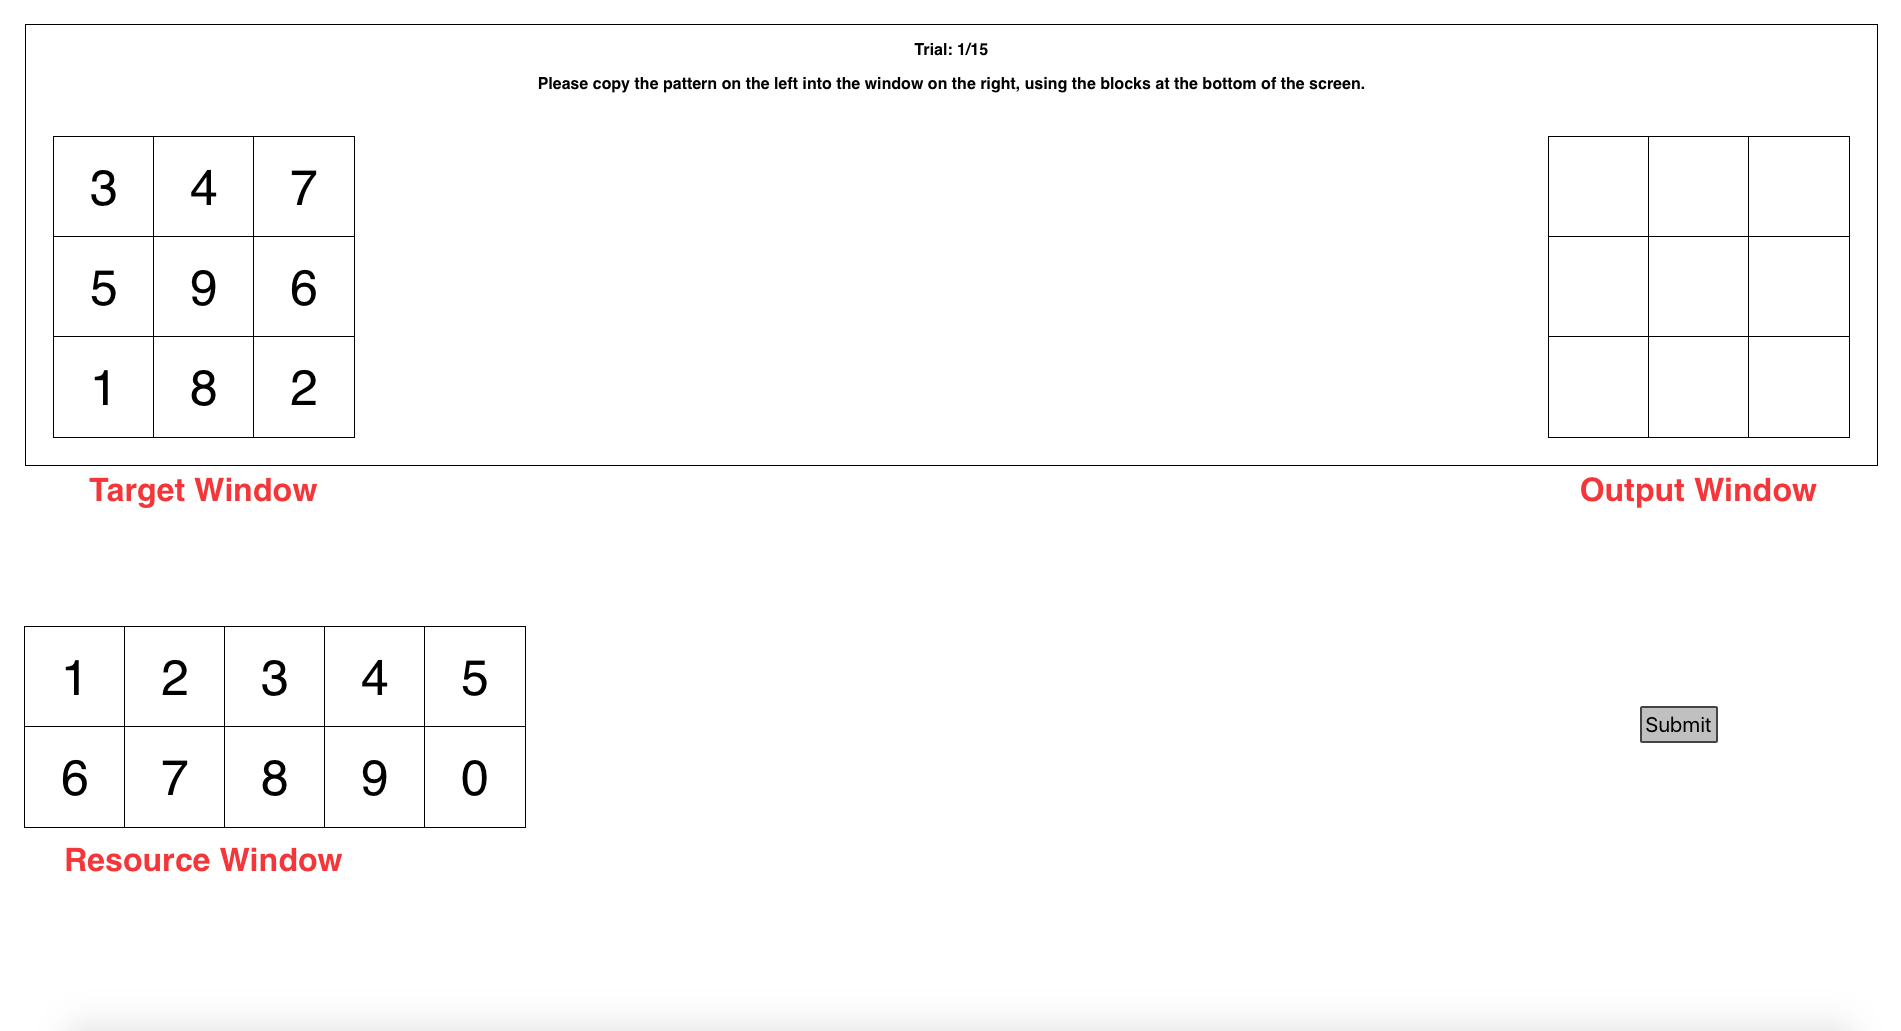
\includegraphics[scale=0.23]{images/Study2/ch4_numbers.png}}
\caption{The number condition.}
\label{fig:ch4_BWT}
\end{subfigure}
%\hfill%
\begin{subfigure}[b]{0.5\textwidth}
\centerline{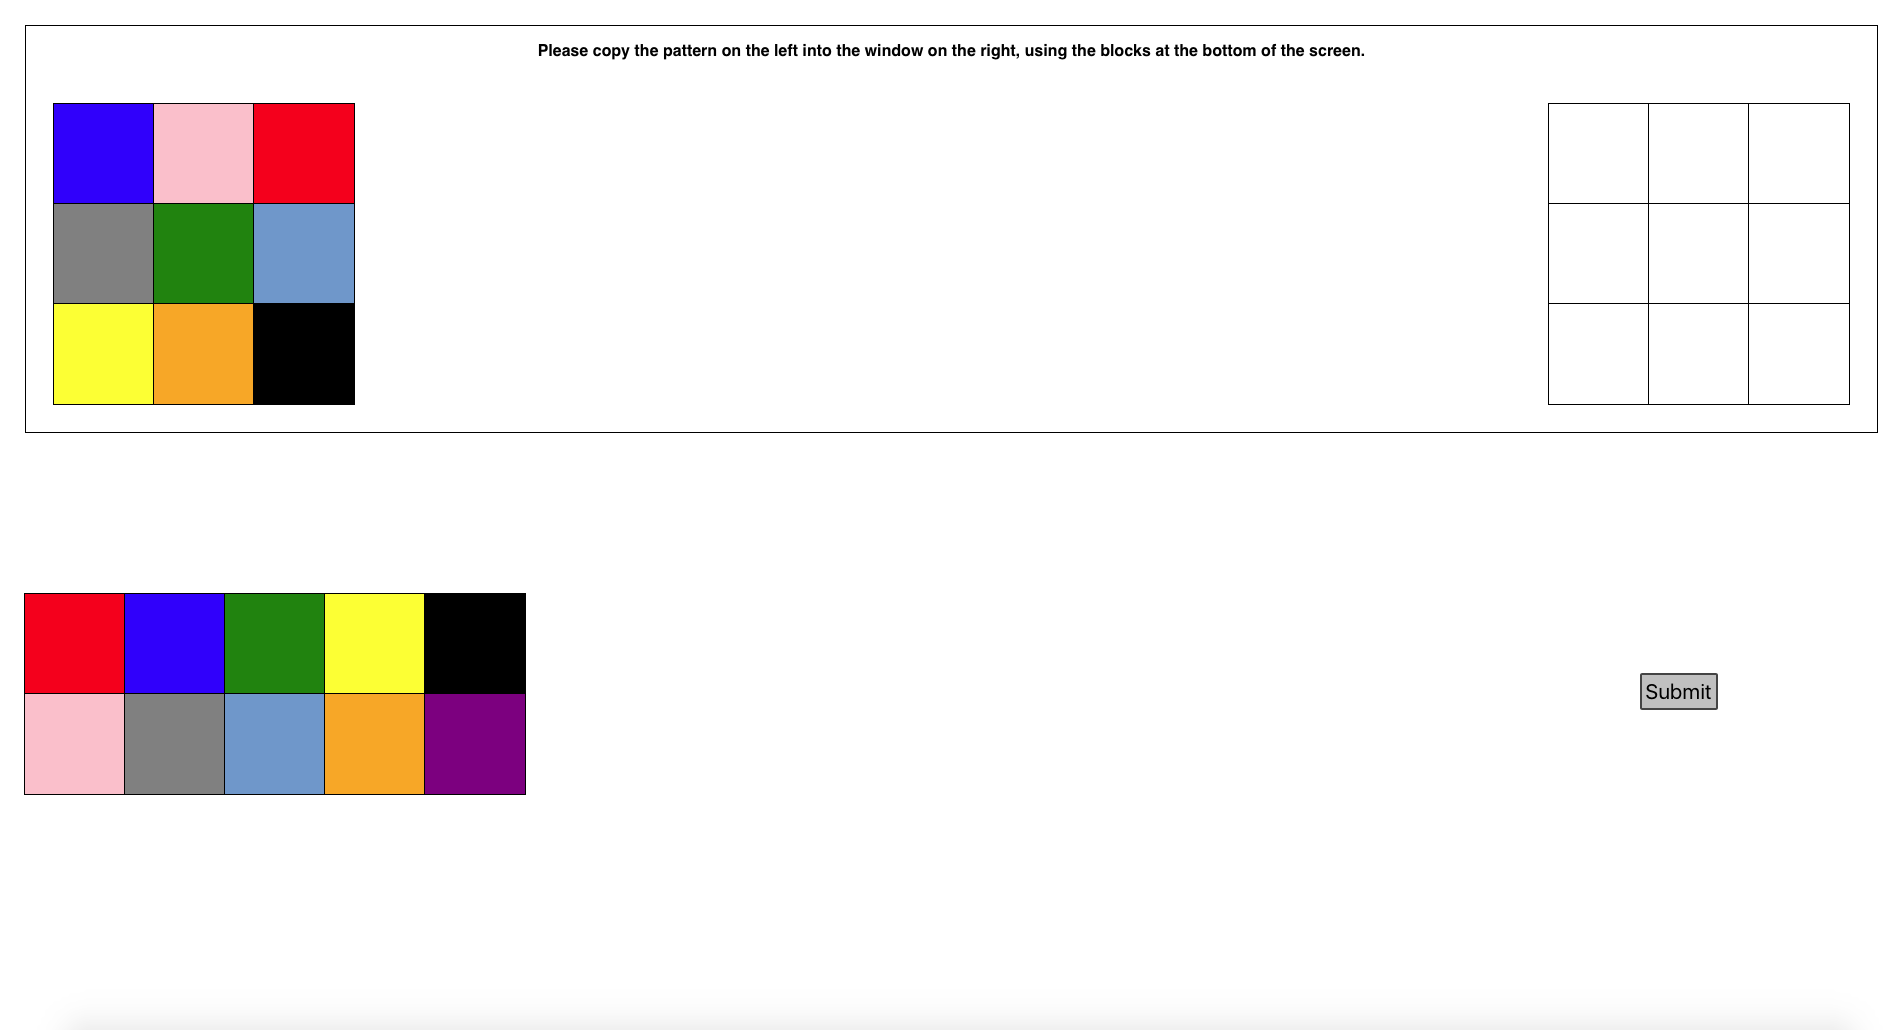
\includegraphics[scale=0.23]{images/Study2/ch4_colours.png}}
\caption{The colour condition.}
\label{fig:ch4_NWT}
\end{subfigure}
\caption[Study 3 task lay-out]{The task lay-out with the three different components.}
\label{fig:ch4_taskparadigm}
\end{center}
\end{figure}

Figure \ref{fig:ch4_taskparadigm} shows the task paradigm that was used. Each colour or number was only used once. The colours used were similar to the colours used in previous BWT studies \citep[e.g.][]{Gray2006, Morgan2009}.
Participants had to copy and complete fifteen patterns of each block type, and each participant had to copy over the same patterns. The target window showed a 3x3 grid with either coloured or numbered blocks. The output window showed an empty 3x3 grid, and was the same size as the target window. Participants had to copy the pattern shown in the target window by dragging blocks from the resource window and moving them into the output window. 

%Apparatus
The study was conducted on a desktop computer, using a 24-inch monitor with a resolution of 2048 x 1152 pixels. Participants used a computer mouse to drag and drop blocks. The experimental task was implemented using HTML, Javascript and PHP and run in a browser.  All relevant browser events, such as mouse movements to (un)cover the grey mask, dragging and dropping the blocks and mouse clicks, were recorded and saved in a mySQL database. The browser window covered the whole screen to minimise distractions.

For the Low IAC condition, eye fixations were used to measure the number and duration of visits to the target window. Eyetracking data was also obtained for the Medium and High IAC conditions. However, this data was not used due to the fact that people were able to also view the target window area whilst the target pattern was covered. Therefore, in accordance with previous IAC studies \citep[e.g.][]{Gray2004}, for the Medium and High IAC conditions the number and duration of uncovering the mask was taken as a measurement for visits to the target window.  These uncoverings were measured by Javascript. The usefulness and limitations of using these measures are discussed in the Discussion.

A Tobii T60 eyetracker was used for recording people's eye fixations. Eye movements were recorded at a rate of 60 gaze data points per second for each eye, with an accuracy of 0.5 degrees and timestamp accuracy of 4 ms. For the analysis, all consecutive eye fixations with no drag or drop actions in-between were added together and counted as one fixation.

\subsubsection{Procedure}
Participants were welcomed and briefed about the experiment. It was explained they would be shown nine blocks which were in a certain order, and had to copy this order by moving blocks around. Participants were instructed to complete the task as fast as possible, but it was explained that they were not able to continue until they had copied a pattern correctly. 
The experiment was broken down in two parts, one where they had to copy colours, and one where they had to copy numbers. For each part, they were given two practice trials first to get familiar with the set-up, and to give them a chance to ask questions if anything was unclear. There was an opportunity for the participant to take a break between the two parts. 
They were then asked to read and sign a consent form and given an information sheet with a summary of the study and the researcher's contact details. In addition to the verbal briefing, the explanation of the study was written out on the computer screen for the participant to read and they were shown an instruction video that showed how the experiment worked. The study took around 20-30 minutes to complete.

\subsubsection{Ethical considerations}\label{sec:quanethics}
The study was undertaken with ethical approval from the UCL Research Ethics Committee [Project ID Number UCLIC/1415/001/Staff Brumby/Borghouts]. 
At the start of each study, participants were first briefed verbally about the study. They were asked to read and sign a consent form, and were given an information sheet to keep. This information sheet contained a summary of the study information and the researchers' contact details. It was explained that an eyetracker would record their eye fixations and movements, but that these recordings were anonymous and that they would not be directly identifiable. After participants had completed the first part of the experiment, a prompt appeared on the screen advising them to take a short break. Participants could take a break as long as they wanted and could decide themselves when to continue with the second part of the experiment.

Participants were informed that the data would be used for research purposes only and stored in accordance with the Data Protection Act 1998. They were also informed that their data would be anonymised and when used in a report or academic paper, their data would not be directly identifiable. 
 
\subsection{Results}
The means and standard deviations of all dependent variables are shown in Table \ref{table:ch4_IACmeans}.

Eight participants were removed from the analysis due to weak eye-tracking calibration. Furthermore, one participant misunderstood the experiment and did not know she was allowed to uncover the mask of the target window more than once. This participant had scores that were more than three times the interquartile range from the rest of the participants' scores on six different variables, so this participant was considered an outlier and removed from the analysis. 


\begin{table*}\centering
\ra{1.3}
%\begin{tabular}{|p{6cm}|lll|lll|}\toprule
\begin{tabular}{@{}p{6cm}lllclll@{}}\toprule
%\begin{tabular}{  p{6cm} l p{1cm} l p{2cm} l  p{1cm}l p{1cm} | p{2cm} | p{1cm}|}
 & \multicolumn{3}{c}{\textbf{Colours}} & \multicolumn{3}{r}{\textbf{Numbers}} \\
 \cmidrule{2-4} \cmidrule{6-8}
 & Low & Medium & High && Low & Medium & High\\\midrule
\textbf{Strategy measures}\\
Number of visits to target window & \textbf{6.36} & \textbf{4.24} & \textbf{2.98} && \textbf{5.10} & \textbf{2.03} & \textbf{2.05} \\
						    & 		    2.28 & 		1.62   & 	          0.90 && 		2.48   & 	         0.63  & 	       0.67 \\
Visit time of first visit (s)  		    & \textbf{0.39} & \textbf{0.04} & \textbf{2.18} && \textbf{0.51} & \textbf{0.04} & \textbf{1.49} \\
				       		    &              0.23   & 		  0.02  & 	         1.59  && 		 0.45  & 	         0.05 & 	      1.01 \\
Average time of visits (s)  		    & \textbf{0.29} & \textbf{0.04} & \textbf{1.54} && \textbf{0.35} & \textbf{0.04} & \textbf{1.07} \\
				       		    &              0.13   & 		  0.02  & 	         0.95  && 		 0.15  & 	         0.03 & 	      0.77 \\
Number of blocks copied		    & \textbf{1.90} & \textbf{3.55} & \textbf{4.52} && \textbf{2.44} & \textbf{6.18} & \textbf{6.33} \\
 after first visit 		       		    &              1.84   & 		  1.93  & 	         1.43  && 		 1.89  & 	         1.61 & 	      1.67 \\
Number of blocks copied correctly & \textbf{1.86} & \textbf{3.22} & \textbf{4.07} && \textbf{2.36} & \textbf{5.96} & \textbf{5.98} \\
after first visit 		       		    &              1.75   & 		  1.83  & 	         1.20  && 		 1.74  & 	         1.52 & 	      1.55 \\

\vspace{10pt}

\textbf{Global task performance measures}\\
Number of incorrectly placed blocks 
				  		    & \textbf{0.15} & \textbf{0.67} & \textbf{0.79} && \textbf{0.17} & \textbf{0.31} & \textbf{0.46} \\
(per trial) 				       	    &              0.18   & 		  0.40  & 	         0.44  && 		 0.19  & 	         0.18 & 	      0.16 \\
Number of incorrectly submitted
				  		    & \textbf{0.27} & \textbf{1.9} & \textbf{2} && \textbf{0.36} & \textbf{0.5} & \textbf{0.83} \\
trials (per experiment block)	    &              0.65   & 		2.51 & 	   2.13  && 		 1.21  & 	         1.08 & 	      1.03 \\
Trial completion time incl. lockout
				  		    & \textbf{19.60} & \textbf{25.40} & \textbf{31.80} && \textbf{19.47} & \textbf{20.83} & \textbf{25.95} \\
(s)						    &                2.98   & 		5.16 & 	   	     6.08  && 	         3.03  & 	        3.08   & 	         4.21 \\
Trial completion time excl. lockout
				  		    & \textbf{19.60} & \textbf{25.40} & \textbf{28.84} && \textbf{19.47} & \textbf{20.83} & \textbf{23.89} \\
(s)						    &              2.98   & 		5.16 & 	   6.34  && 		 3.03  & 	         3.08 & 	      4.06 \\

\bottomrule
\end{tabular}
\caption[Study 3 descriptive measures]{The effect of IAC on copying colours and numbers. The means are shown in bold, the standard deviations are below the means.}
\label{table:ch4_IACmeans}
\end{table}

\subsubsection{Task strategies}

\subsubsection{Number of visits to the target window}
Participants made fewer visits to the target source when they had to copy numbers (M = 3.06, SD = 2.08) than when they had to copy colours (M = 4.49, SD = 2.18), F(1,30) = 41.62, p<.001, $\eta^2$  = 0.58. Participants also made fewer visits as IAC increased from Low (M = 5.73, SD = 2.41), to Med (M = 3.13, SD = 1.65), to High (M = 2.51, SD = 0.91), F(2,30) = 15.16, p<0.001, $\eta^2$  = 0.50. To investigate differences between conditions, post-hoc Tukey comparisons were performed. Results showed that participants made significantly fewer visits in the Medium-IAC condition than in the Low-IAC condition, p <.01. However, there was no difference in number of visits between the Medium-IAC and the High-IAC conditions, p=.59. Participants looked at the target window for colours more on every level of IAC (see Figure \ref{fig:ch4_noVisits}), and so there was no significant interaction, F(2,30) = 2.82, p=.08, $\eta^2$  = 0.16. 

\begin{figure}[!ht]
\centering
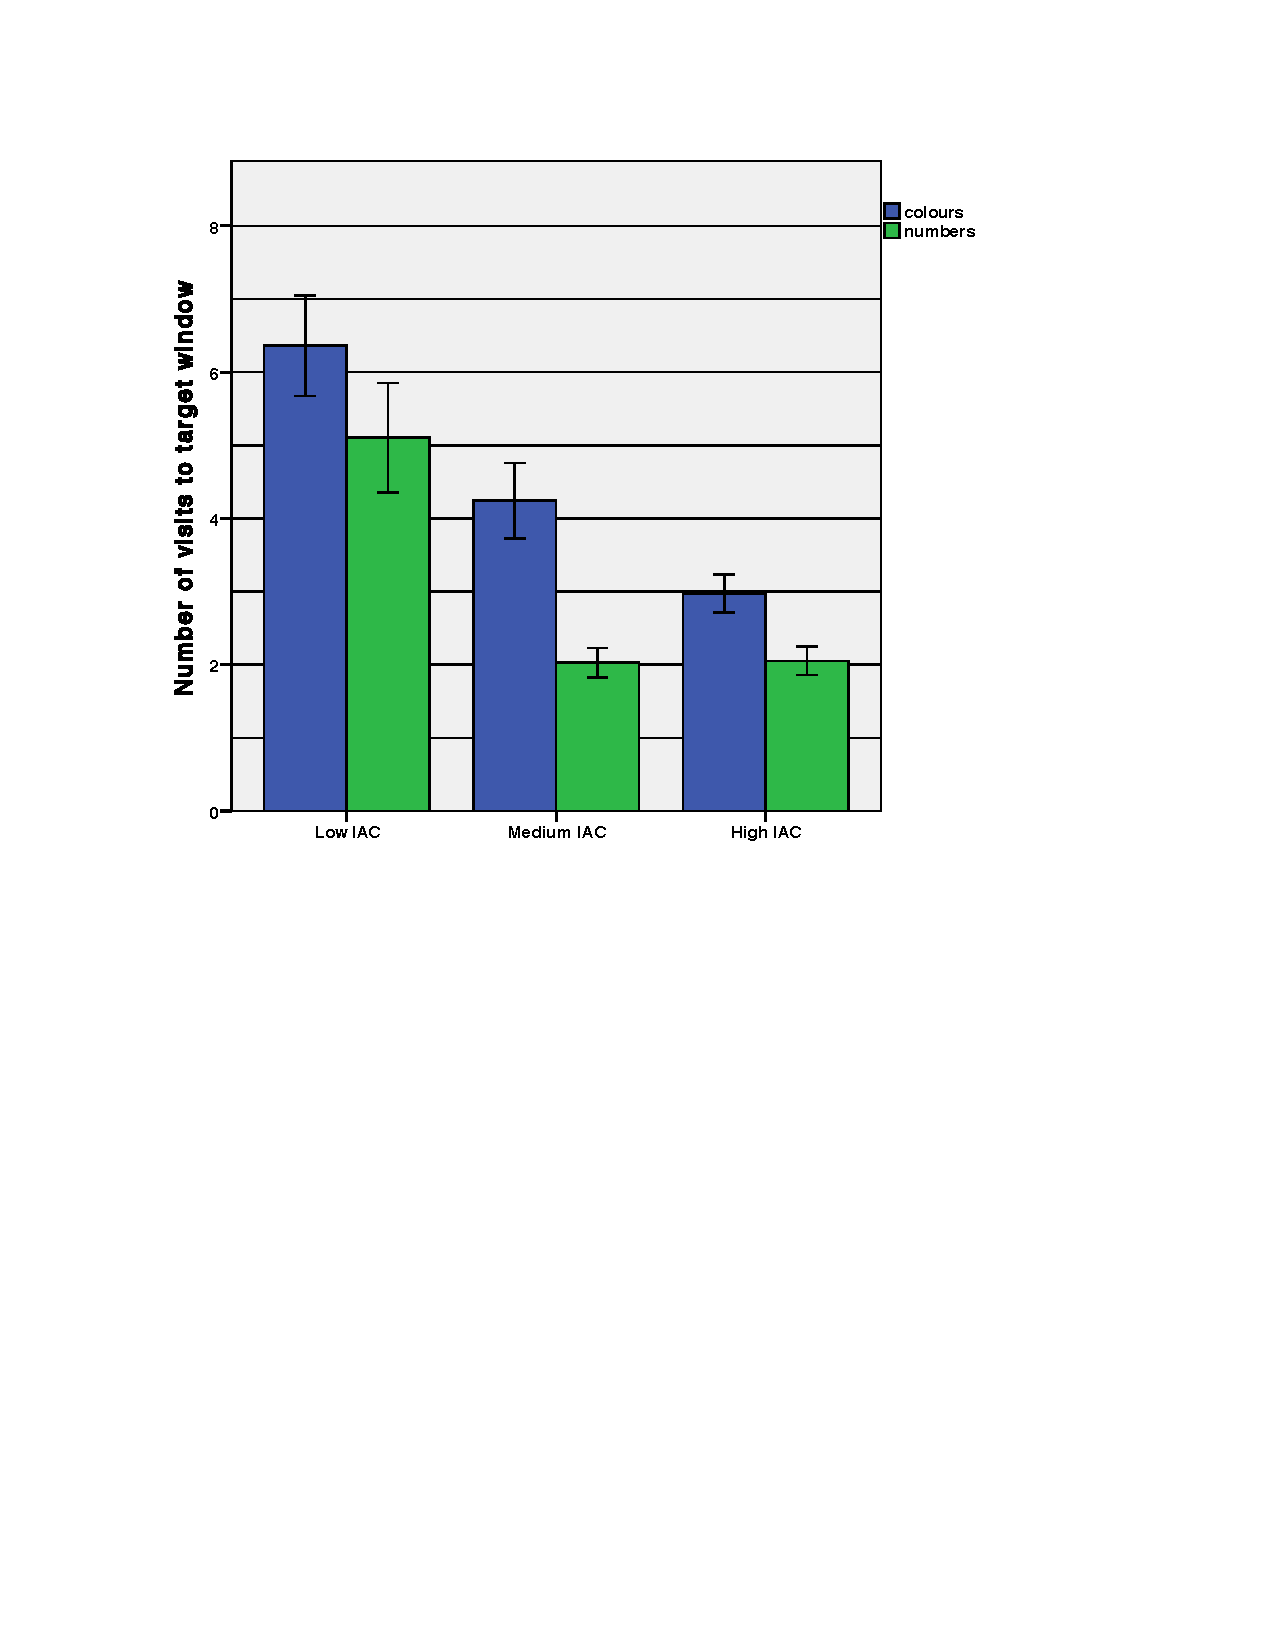
\includegraphics[width=\textwidth]{images/Study2/ch4_noVisits-bargraph.pdf}
\caption[Study 3 number of visits]{The interaction between block type and IAC for number of visits to the target window. The error bars represent $\pm $1 standard error.}
\vspace{-9pt}
\label{fig:ch4_noVisits}
\end{figure}

\subsubsection{Duration of first visit to target window}
There was no significant main effect of block type on the duration of the first visit, F(1,30) = 3.05, p=.09, $\eta^2$  = 0.09. Participants looked longer at the target source as IAC increased from Low to High. Post-hoc comparisons showed that participants looked longer in the High-IAC condition (M=1.84, SD = 1.35) than in the Low/Medium-IAC conditions, ps <.001. However, there was no difference in duration between the Low-IAC (M = 0.45, SD = 0.46) and the Medium-IAC (M = 0.05, SD = 0.04) conditions, p=.47. There was a significant interaction effect between IAC and block type, F(2,30) = 5.70, p<.01, $\eta^2$  = 0.28 (see Figure \ref{fig:ch4_firstVisitDuration}). There were no difference between block types in the Low-IAC condition, t(10) = -1.86, p = 0.09, nor the Medium-IAC condition, t(9) = -0.29, p = 0.7. However, in the High-IAC condition, participants looked significantly longer for colours (M = 2.18, SD = 1.59) than numbers (M = 1.49, SD = 1.01), t(11) = 2.76, p = 0.02.

\begin{figure}[!ht]
\centering
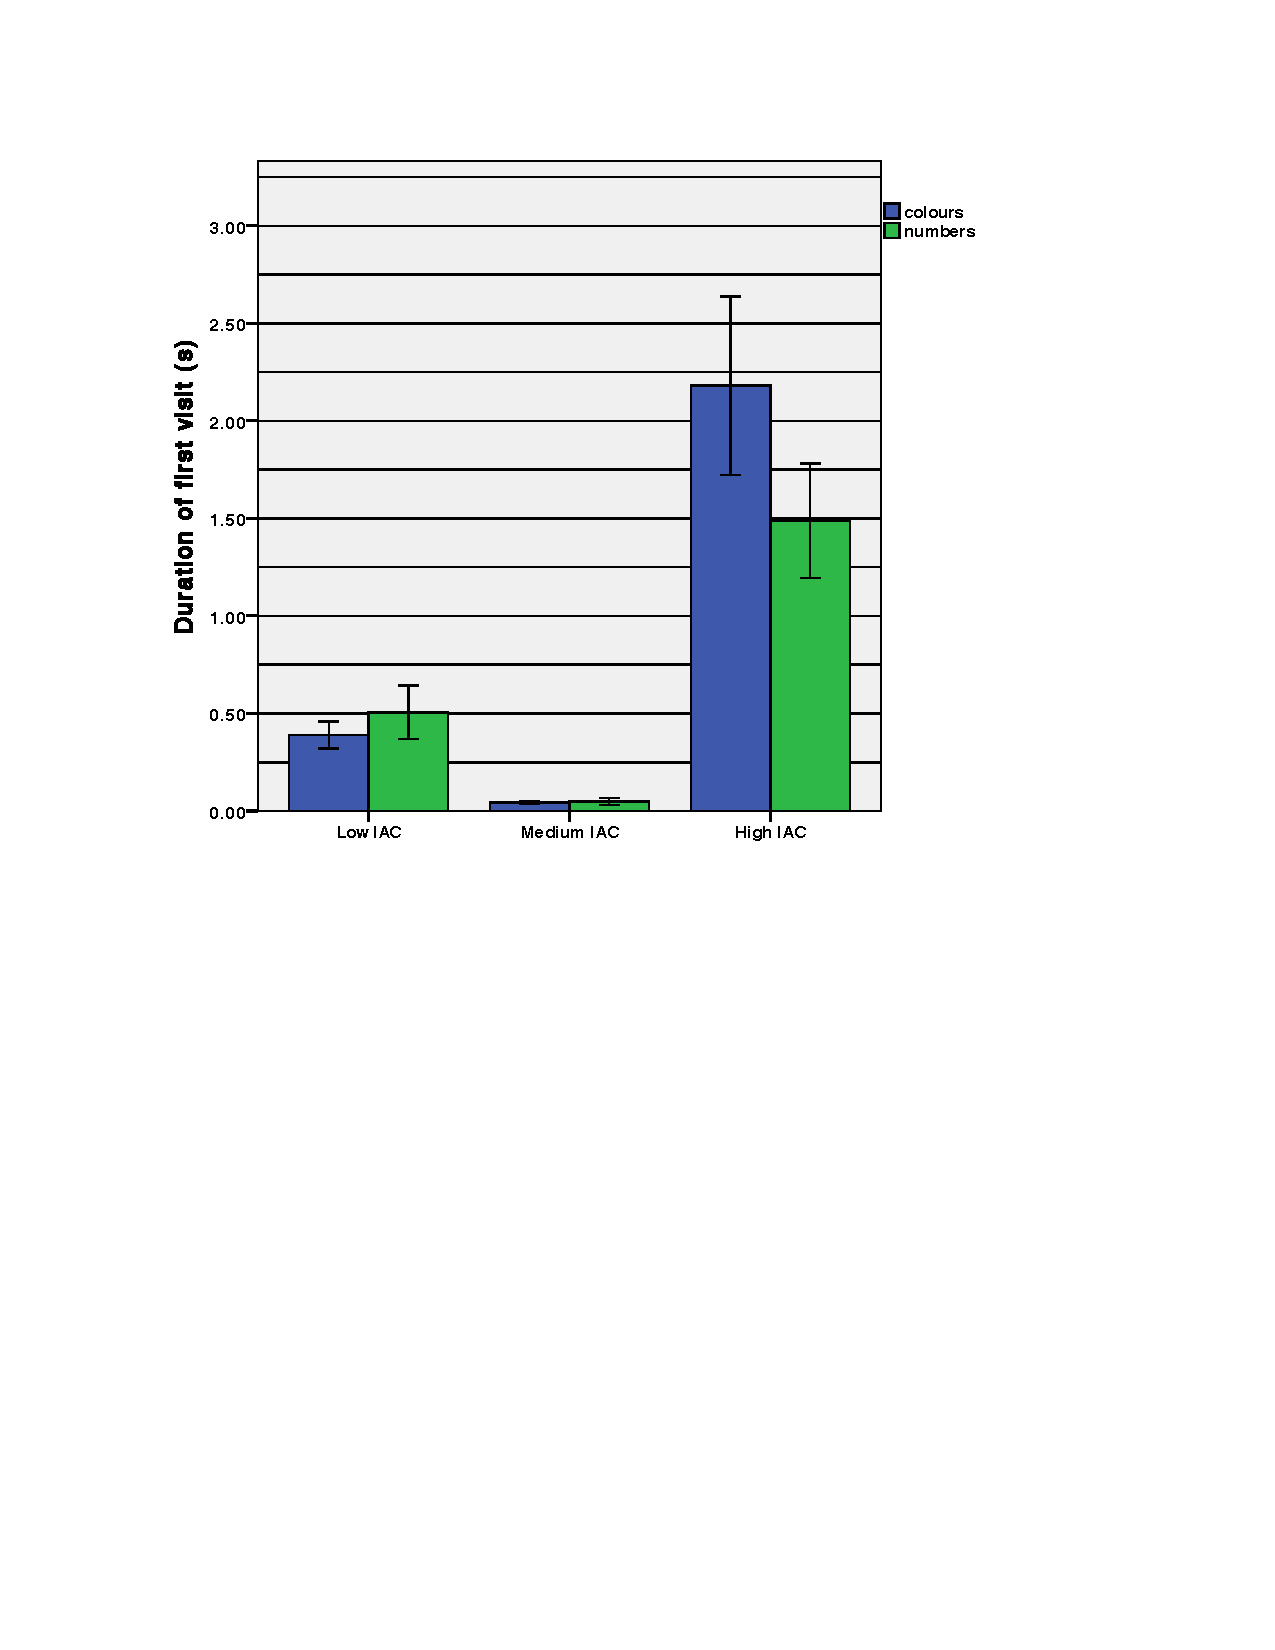
\includegraphics[width=\textwidth]{images/Study2/ch4_firstVisitDuration-bargraph.pdf}
\caption[Study 3 duration of first visit]{The effect of IAC on the duration of the first visit to the target window. The error bars represent $\pm $1 standard error.}
\vspace{-9pt}
\label{fig:ch4_firstVisitDuration}
\end{figure}

\subsubsection{Blocks placed after first visit}
People placed more blocks correctly after the first visit for numbers (M = 4.77, SD = 2.33) than colours (M = 3.08, SD = 1.81), F(1,30) = 63.86, p<.001, $\eta^2$  = 0.68. They also placed more blocks as IAC increased, F(2,30) = 12.54, p<0.001, $\eta^2$  = 0.46. Tukey post-hoc comparisons show there was a difference between the Low IAC and Medium/High IAC conditions (ps<.01), but not between Medium and High IAC conditions (p=.77). There was a significant interaction effect between IAC and block type, F(2,30) = 8.96, p<.01, $\eta^2$  = 0.37  (see Figure \ref{fig:ch4_firstCorrectBlocks}). When IAC was Low, the number of blocks that were copied correctly after the first visit did not differ significantly for colours or numbers.

\begin{figure}[!ht]
\centering
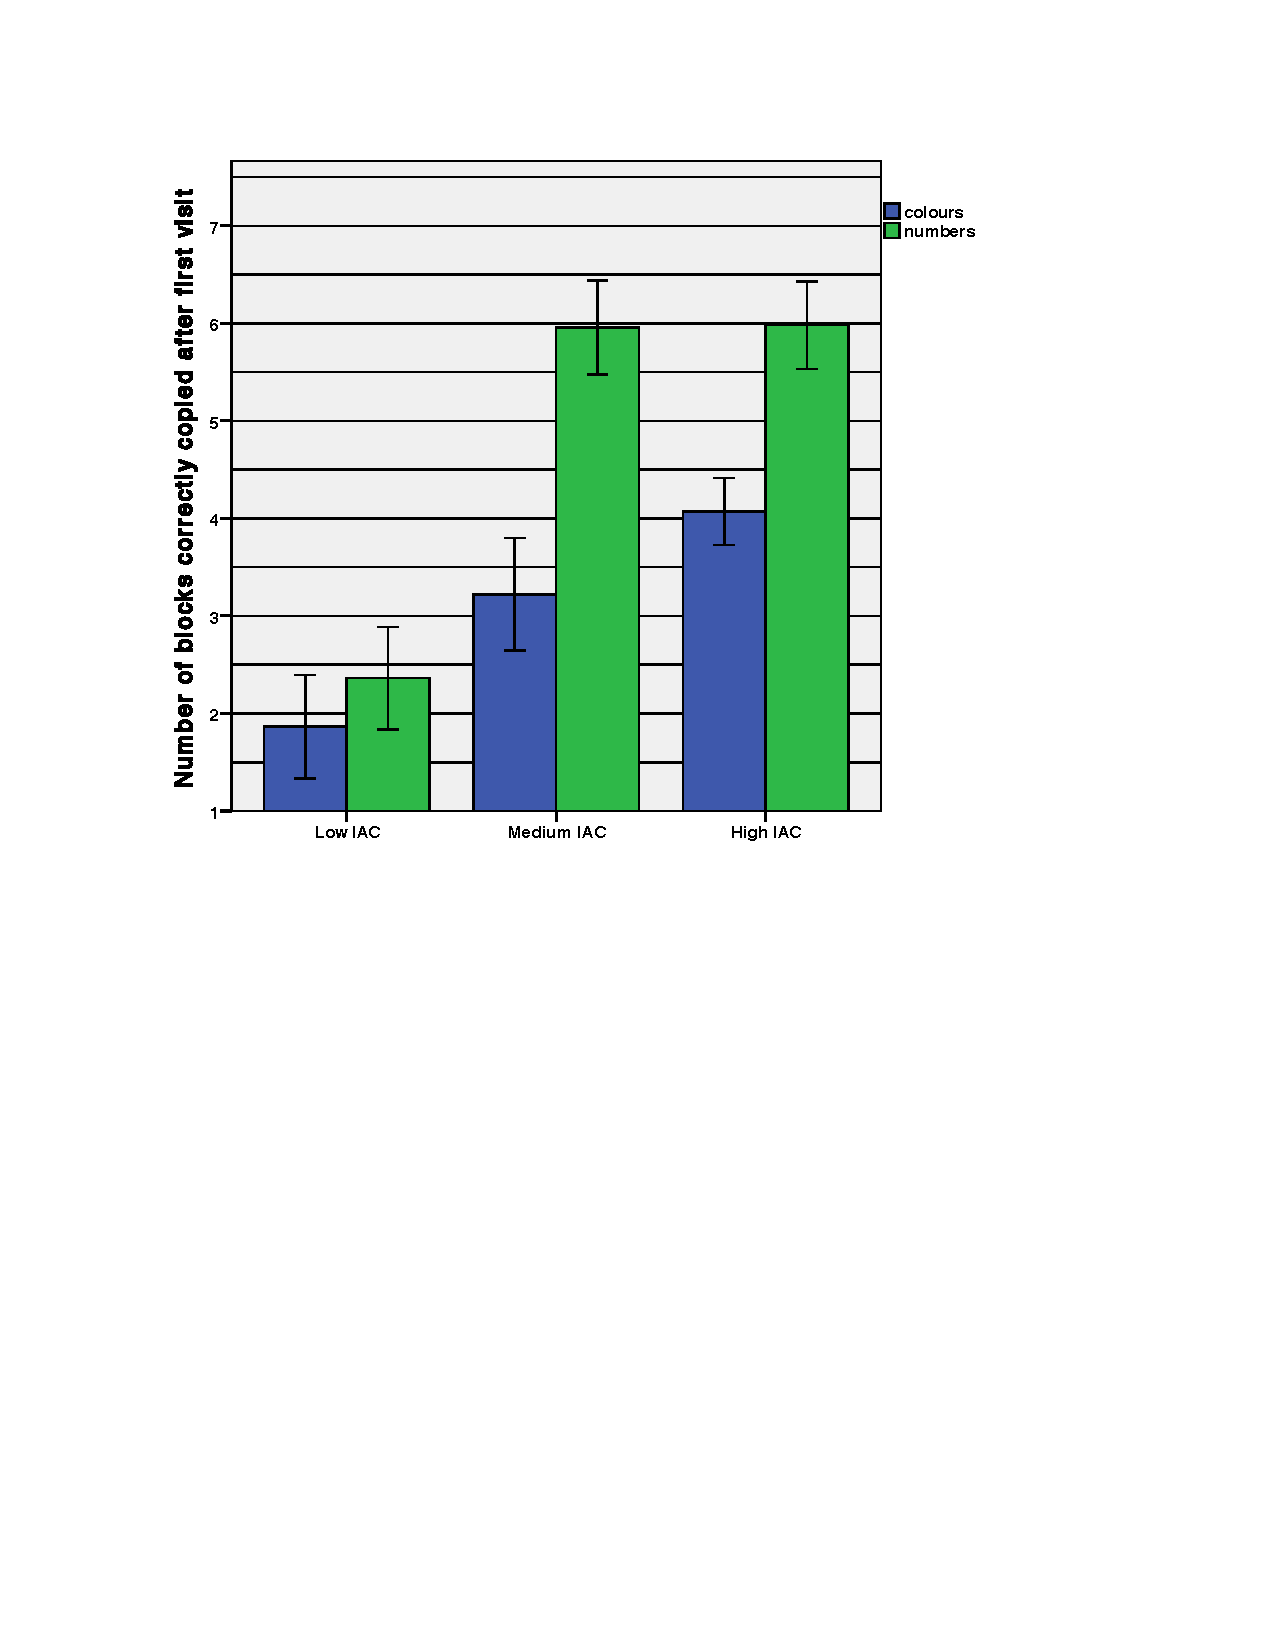
\includegraphics[width=\textwidth]{images/Study2/ch4_firstCorrectBlocks-bargraph.pdf}
\caption[Study 3 number of blocks correctly placed]{The interaction between block type and IAC for number of blocks correctly placed after the first visit to the target window. The error bars represent $\pm $1 standard error.}
\vspace{-9pt}
\label{fig:ch4_firstCorrectBlocks}
\end{figure}

\subsubsection{Global task performance}
The interactions between block type and IAC on global task performance measures all had the same trend: people performed the same for colours and numbers when IAC was Low, but differences appeared between the block types as IAC increased. As this trend was the same for each interaction, the statistical results of the interactions are reported but their specific trend will not be repeated.

\subsubsection{Number of incorrectly placed blocks}
Participants placed more blocks incorrectly for colours (M = 0.54, SD = 0.45) than numbers (M = 0.32, SD = 0.21), F(1,30) = 10.71, p=.003, $\eta^2$ = 0.26. As IAC increased and participants were keeping more items in memory, they increasingly placed more incorrect blocks, F(2,30) = 14.71, p<.001, $\eta^2$ = 0.50. Tukey post-hoc comparisons show there was a difference between the Low IAC condition (M = 0.16, SD = 0.18) and Medium/High IAC conditions (ps<.01), but not between the Medium (M = 0.49, SD = 0.35) and High IAC conditions (M = 0.63, SD = 0.36) (p = .3). There was a significant interaction effect between IAC and block type, F(2,30) = 3.36, p<.05, $\eta^2$ = 0.18. When IAC was Low, the number of blocks that were copied incorrectly did not differ significantly for colours or numbers, but as IAC increased, participants placed more blocks incorrectly for colours.

\subsubsection{Number of incorrectly submitted trials}
The number of trials that were submitted incorrectly was generally low, but participants submitted more incorrect trials for colours (M = 0.1, SD = 0.16) than numbers (M = 0.04, SD = 0.08), F(1,30) = 5.28, p=.029, $\eta^2$ = 0.15. There was no significant effect of IAC, F(2,30) = 2.70, p=0.08, $\eta^2$ = 0.15, nor any interaction, F(2,30) = 1.65, p=.2, $\eta^2$ = 0.10.

\subsubsection{Trial time}
Two trial completion times are considered here: total time and time excluding lockout. 
Looking at the actual completion time, participants took longer to complete a trial when they were copying colours (M = 25.80, SD = 7.06) compared to when copying numbers (M = 22.24, SD = 4.47), F(1,30) = 44.08, p<.001, $\eta^2$ = 0.60. As IAC increased from Low to Medium to High, participants took longer to complete a trial, IAC, F(2,30) = 15.91, p<0.001, $\eta^2$ = 0.52. Tukey post-hoc comparisons show there was a difference between Low/Medium and High (ps<.01), but not between Low and Medium (p = .12). There was a significant interaction effect between IAC and block type, F(2,30) = 11.05, p<.001, $\eta^2$ = 0.42. 

With the lockout time in the High-IAC condition removed, the same effects were found for block type, F(1,30) = 34.55, p<.001, $\eta^2$ = 0.54, and IAC, F(2,30) = 8.18, p=0.001, $\eta^2$ = 0.35. Tukey post-hoc comparisons show there was still a difference between Low and High (p=.001), but no longer between the Medium IAC and Low IAC or High IAC conditions (ps >.1). There was a significant interaction effect between IAC and block type, F(2,30) = 8.13, p=.002, $\eta^2$ = 0.35.

\subsubsection{Qualitative data}
The screen recordings from the eye-tracker were played back to further investigate people's behaviour. Although this helped understand some behaviour which could not be determined from the quantitative data alone, these observations only serve to explain some of the quantitative measures and are not the main focus of the analysis.

The visit durations in the Medium IAC condition were suspiciously short. Upon replaying the screen recordings, it appeared that participants often accidentally moved their cursor over the grey mask of the target source. This was counted as a visit by the program, even though participants may have not intentionally moved their cursor to this part of the screen to look at the target source. They did not spend a long time looking at the target window, but also did not immediately move blocks either, and sometimes waited multiple seconds before they made a move. 

\begin{figure}[!ht]
\centering
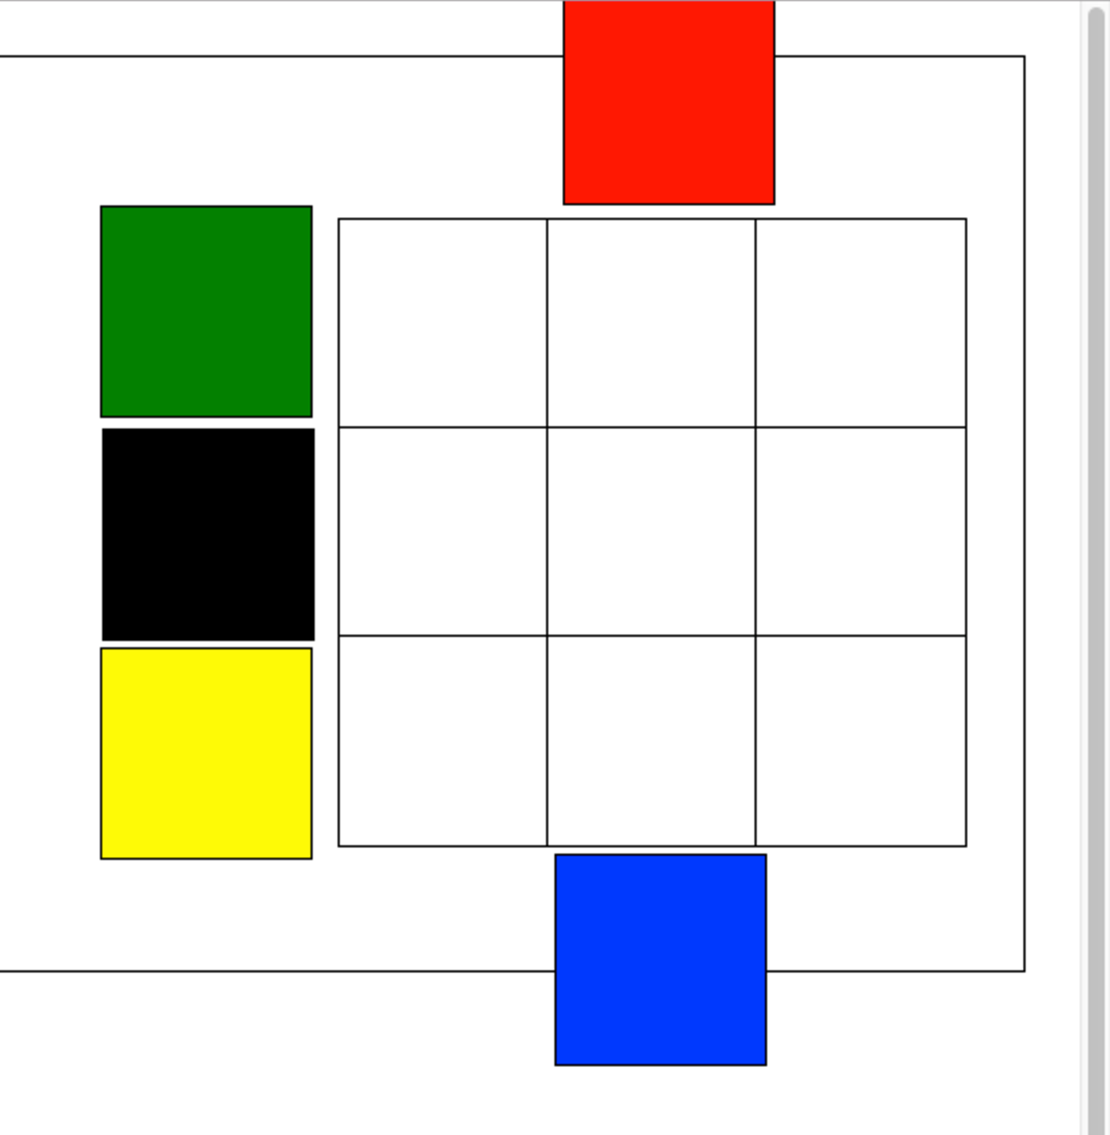
\includegraphics[scale=0.3]{images/Study2/ch4_placeholders.pdf}
\caption[Study 3 placeholders]{Participants placed blocks outside of the output window as `placeholders'.}
\vspace{-9pt}
\label{fig:ch4_placeholders}
\end{figure}

During the 1-s lockout in the High IAC condition, participants changed their minds about visiting the target window on numerous occasions. They placed their mouse cursor on the mask, but left this field before it was uncovered to move one or more blocks. It could be this decision also occurred in the Medium IAC condition, but as there was no lockout the mask was already uncovered before people made this decision, and would explain the very short visits.

People sometimes placed the blocks as `placeholders' as shown in Figure \ref{fig:ch4_placeholders}: they placed several blocks outside of the output window next to the position they thought it belonged to, but did not place it there yet. Only after viewing the target again, they placed the blocks in the output window. Looking at quantitative data alone, this type of strategy would be depicted as one long view at the target, after which all blocks were placed in one go. This is true to some extent, but as people could already place the blocks and offload their memory without this being recorded by the program, they only had to check if this position was correct on the subsequent visit, and is different from a strategy where people spent a long time trying to memorise the blocks after which all blocks were placed.


\newpage

\subsection{Discussion}
This study replicated the Blocks World Task with the aim to see if the effect on IAC on a copying task, as previously found when using colours, can be extended to copying numbers, and if a deeper encoding of numbers into memory makes people more accurate.

The main findings are:

\begin{itemize}
\item
Numbers are easier to copy than colours, but only if IAC is increased
\item
Increases in IAC make people adopt memory-intensive strategies
\item
Increases in IAC increases errors
\end{itemize}

\subsubsection{The effect of block type on task strategies and performance}
Changing the block type from colours to numbers made it easier to memorise the blocks: people made shorter and fewer visits than when copying colours, but were still able to place more blocks. This difference in performance is only found in the Medium and High IAC conditions, which further suggests the difference between numbers and colours is due to the memorability of the information, and the interactions on most of the dependent variables further show that the difference between block types was dependent on the level of IAC.

The difference between numbers and colours fit well with the distinction in Baddeley's \citeyearpar{Baddeley1986} seminal model of working memory between processing visuo-spatial and verbal information. As numbers can be rehearsed and therefore refreshed in working memory, they are likely easier to memorise. After the study had ended, several participants in this study explained they used some sort of rehearsal and tried to say the numbers out loud in their head. For colours, some indicated they tried to either capture a mental picture of the colours in their mind, while others rehearsed the word for each colour (e.g. 'red' and 'blue') but they felt they were able to remember fewer items using this strategy. This is consistent with \citet{Chincotta1999}'s finding that people have a greater memory span for Arabic numerals (e.g. 1, 2, 3) than corresponding words (e.g. one, two, three).

Though an increase in IAC made people rely on memory and people seemed to memorise numbers more easily than colours, an increase in IAC did not make people more accurate in copying numbers as in \citet{Gray2004}, where people had to memorise VCR programming information. The error rate for numbers was however already quite low in all conditions, and moreover people were not explicitly instructed or trained to memorise the information before each trial as in \citet{Gray2004}.

\subsubsection{The effect of IAC on task strategies and performance}
The effect of IAC on people's cognitive strategies, as found in previous studies, is replicated in this study: as the cost of accessing the target window increased, people increasingly relied on memory \citep{Gray2006, Morgan2009, Waldron2007}. People switched from a perceptual to a memory-based strategy by making fewer but longer visits to the target window and placing more blocks immediately after the first visit. This strategy worsened their global performance as they took longer to complete the task and placed more incorrect blocks throughout the trials. 

An increase in IAC also made people rely more on memory when copying numbers. When a mask was added over the target window, people visited the target window less often and they placed more blocks after the first visit. In both the Medium IAC and High IAC conditions, people on average placed around six blocks correctly after the first visit, after which they needed one more visit to look at the last three blocks. The average number of items people can memorise is 7$\pm$2 items \citep{Miller1956}, and potentially six blocks was the maximum that people could reasonably memorise.

In previous studies, adopting a memory-based strategy when copying text and numbers improved accuracy \citep{Gray2004, Soboczenski2013}. In the current study, the hypothesis that memorising numbers due to an increased IAC would make people more accurate is not supported. 
The error rate was overall low and upon reflection the interaction of moving blocks may have made people sufficiently slow to hardly make any errors. In \citet{Gray2004} and \citet{Soboczenski2013}, people typed in data using a computer keyboard.

With the BWT, it was difficult to measure visits to the target window in the same manner for all conditions. For the Low IAC conditions, eye fixations were used, whereas for the Medium and High IAC conditions, uncoverings of the mask were used. This introduced several problems. First, while eye-tracking measures show how long and how often people are looking at a particular part of the screen, it can not reveal if people are actually perceiving or processing the data that is displayed \citep{Waldron2007}. For the Medium and High IAC conditions, an interaction was required and a conscious decision had to be made to reveal the target in these conditions. It would therefore seem likely that uncoverings more reliably measure visits to the target window. However, the uncoverings for the Medium IAC conditions were suspiciously short. Playing back the screen recordings suggests participants often accidentally uncovered the window, and it is therefore less clear if these are a reliable measure of actual visits. 

\subsubsection{Summary}
The purpose of this study was to study the effect of IAC on strategy, speed and accuracy when copying from one source, and investigate if the effect of IAC, as found in previous experimental studies, would extend to copying numbers. In order to be able to compare results of this study with previous IAC studies the same task paradigm of the Blocks World Task was used.

The hypothesis that people would need fewer switches and would perform better for numbers than colours is supported, indicating that numbers are easier to memorise. The hypothesis that memorising numbers due to an increased IAC would make people perform better is not supported. The error rate was overall low and upon reflection the interaction of moving blocks may have made people sufficiently slow to hardly make any errors. Furthermore, in Study 1 people saved up data to enter a lot in one sequence, and errors increase as people have to copy more \citep{Healy2004}. Potentially the setup of this experiment was not suitable to reliably measure an increase in errors.
 
The information was copied from one source, and for each participant the IAC was the same throughout the experiment: it was either low, medium, or high. Therefore, while using the BWT task paradigm was appropriate in comparing its results with previous IAC studies, it did not resemble the data entry tasks observed in the financial office setting of Study 1. 

Considering these limitations, it was decided after this study to not continue with the same task paradigm, but certain learning points can be taken away from this study.  

First, the entry method matters. An entry method that is sufficiently slow may make people accurate, regardless of the level of IAC. 
Second, the effect of IAC generalises, but it is not clear how the results of this experimental paradigm can be translated in suggestions in how people dealing with differing levels of IAC can best be supported in their work. In contrast to this study, where information came from one source, and always had the same level of IAC for each participant, Study 1 showed that for entering expenses, people have to enter different types of information, these do not all come from the same source, and each source can have a different access cost.

Third, the measured short visits in the Medium IAC conditions may have confounded the results. In future studies, the setup of the experiment should be designed so that participants do not accidentally access the source when they do not intend to.

Lastly, for each dependent variable, the same consistent measure should be used to compare across conditions. This could be data provided by an eyetracker, or interaction measures such as mouse clicks, key presses or interkey intervals. 

The next study will try to more closely simulate the expenses task observed in the financial office setting of Study 1 and 2. People will have to enter and collect information from multiple sources with different IACs. The aim is to see how these differences in IAC influence people's switching strategies between entering and looking up data when copying from multiple sources. 

%In order to be able to further conduct experiments that study how people can best be supported when retrieving information for a data entry task, it is important to understand where they have to get it from. Therefore, the next study I will focus on the expenses task identified in Study 1 and look at the resources people need for this task, where they need to get it from, and how costly it is to access this information.


\section{Study 4: Copying data from multiple sources}
 
\subsection{Introduction}
%Study 3 will have given a better understanding of the expenses task, identified the information sources needed for this task and their levels of IAC, and will have given insight into how people manage subtasks to look up information.
Study 1 and 2 showed that for an expenses task, people have to collect the data to enter from multiple sources. Some of these sources are easy to access such as paper sheets on a desk, while others have a higher IAC, such as a computer document or window that takes time to open and view.

Study 3 has given an understanding of the effect of IAC on people's switching strategies when copying from one information source. As IAC increases, people make fewer visits to the source and instead enter what is in their head. 
The current study aims to investigate how differences in IAC affect people's strategies in switching between entering and looking up information from multiple sources, and whether different strategies affect performance.

The office setting of Study 1 and 2 will be simulated in a laboratory environment. Participants will have to retrieve data from a number of sources, and enter this into a desktop computer using keyboard and mouse. The sources will be made to resemble the sources identified in Study 1 and 2 and will be on paper, on a second computer screen, or on the same screen as where the participant has to enter the data. The data participants have to enter will be similar to data that is entered for an expenses task: this includes names, financial numbers, and alphanumeric strings. 

Study 3 used eyetracking data and mouse movements to measure number and duration of visits to the target source. For the setup in this experiment, these measurements are not possible for visits to paper sources with the eyetracking equipment available.
I will therefore video record and/or observe participants and code the timing and number of visits people make to the different information sources.
To supplement these with quantitative measures, I will also measure keylogging data to get further insight whether and how long people interrupt entering data, presumably to retrieve data. In accordance with \citet{Gould2016}, intervals of more than 5s are considered to be an interruption. 

A within-subjects design will be used. The independent variables will be type of data (e.g. names, financial numbers, and alphanumeric strings), and IAC of the information sources. Dependent variables will be number of visits to sources, timing of visits, resumption lag, interkey intervals, typing speed, and error rate.

It is expected people will develop strategies as they have to enter data over an extended period of time. 
For example, they may initially look up each data item the moment they need it, but as they become familiar with the IAC of sources, they may first finish entering all information from low IAC sources, before looking up information of high IAC sources. 

Office workers from Study 1 and 2 have experience with entering expenses and have found ways to optimise their work. If it is not possible for this user group to participate in the laboratory experiments, I will have to pilot it to see how long the experiment needs to run, in order to allow enough time for participants to exhibit changes in strategies. The same ethical considerations as described in Study 2 (section \ref{sec:quanethics}) will be made, and participants will be given the opportunity to take breaks during the experiment. If the total required duration of the experiment exceeds an hour, the experiment will be broken down in multiple sessions.

The identified behaviour of how people manage looking up information is used to create a set of design recommendations for the current expenses system, which are evaluated in Study 5 and 6.

\subsubsection{Hypotheses}
Based on previous IAC studies and findings from Study 3, the following hypotheses can be made: 
\begin{itemize}
\item
As IAC increases, people try to memorise and copy over more data from one source in one go. 
\item 
People will look longer at a high IAC source than a low IAC source.
\end{itemize}
This means that people will interrupt from entering data into the computer to look up information a longer time for a high IAC source than a low IAC source. Studies have shown that the longer people are interrupted from a primary task, the slower they are to resume that task after the interruption \citep[e.g.][]{Monk2008}. Based on this, the following hypothesis is made:
\begin{itemize}
\item 
People will be slower to resume the entry task after retrieving data from a high IAC source than a low IAC source.
\end{itemize}
The soft constraints hypothesis predicts that people choose and adapt their task strategies in order to minimise time. Based on this theory and findings from Study 1 that people try to save up data entry tasks to enter them in one sequence, the following hypothesis is made: 
\begin{itemize}
\item 
As the experiment progresses and people become aware how costly it is to access certain sources, they will learn and choose to enter all the low-IAC items first, in a batch, and then the high-IAC items second, also in a batch, rather than looking up each item as they need it. 
\end{itemize}

\subsubsection{Contributions}
Demonstration that:
\begin{itemize}

\item   
IAC also affects people's strategies of switching between entering and looking at the target source when multiple sources are involved.
\item
IAC affects how people manage subtasks of looking up information in a data entry task.
\item
Depending on users' experience and awareness of how costly it is to access information, they optimise costs by processing all the low-IAC tasks first, in a batch, and then the high-IAC tasks second, also in a batch, rather than switching between the two different types of task.  
\end{itemize}

\chapter{Evaluating design changes to improve performance in data entry with varying IACs}

\begin{mynote}
\subsubsection{Chapter outline}
The previous chapter demonstrated that IAC affects how people switch between entering and looking up information. This chapter describes two studies that, given varying IACs, explore the extent to which design changes to the data entry interface can influence strategies, speed and accuracy. Study 5 evaluates these in a controlled setting, to see if making design changes influence the strategies people adopt, and can make people adopt more accurate and/or efficient strategies. Study 6 evaluates them in the office setting, to ascertain how appropriate the proposed recommendations are in the context in which they would be used.

Together these studies intend to show that the new interface makes people switch less between entering and looking up information, which makes them faster to complete the data entry task overall and can reduce errors.
\end{mynote}

\section{Introduction}

The findings of the previous studies will have given insight into the influence of IAC on people's strategies of managing looking up information and how different strategies may be more efficient and accurate than others. For example, one finding can be that people who look up information from high IAC sources as they need it are slower and make more data entry errors than people who first collect all information and then enter it all in one sequence. 
It will have highlighted some functionalities that a data entry expenses system needs to offer users. These findings are translated into a set of requirements. These are used to test the existing system against, and used to develop possible future design recommendations suited to the task of entering expenses. 

The design recommendations will take into account both findings from Study 3 and 4 on what influences people's strategies and what is desirable, as well as the setting studied in Study 1 and 2 and what is feasible. For example, desired changes in the actual interface may be too expensive to be realistic, and it may be more feasible to change the way information sources are designed, or how these are laid out in the user's environment. Screenshots of the current interface system will be used (initial ones were obtained in Study 1, additional ones will be obtained in Study 2). 

Study 5 aims to test different designs in a controlled experiment, to investigate if changing design features influences people's switching strategies and their speed and accuracy in data entry. It will use the same task paradigm as Study 4 and compare different designs, to see if these changes have an influence on the strategies people adopt in looking up information for a data entry task, and whether these changes can make people adopt strategies that improve accuracy. 

Study 6 aims to evaluate the design recommendations in a finance office with workers, to see how appropriate and feasible the proposed recommendations would be in the context for which they are developed. Depending on what the design recommendations will be, I will take them through a prototype, which can be a paper prototype, storyboard, or digital mockup, and if possible I will ask them to perform the task with and without the proposed changes. 

\subsection{Contributions}
\begin{itemize}
\item
Development of design recommendations for an expenses system.
\item
Demonstrate how an understanding of the used information sources and people's switching strategies between entering and looking up information can be used to adapt the design of the data entry interface. 
\item
Demonstrate the applicability of design recommendations in the financial office settings in which the expenses task is currently done. 
\item
Demonstrate that design features can influence people's strategies in entering expenses in a financial office setting.
\end{itemize}

\bibliographystyle{apacite}
\bibliography{Thesis}

\appendix\label{ch:appendix}
\chapter{Information sheet}\label{ch:information_sheet}
The information sheet given to the participants in Study 1 is shown in Figure \ref{fig:informationsheet}. 

\begin{figure}[htp] \centering{
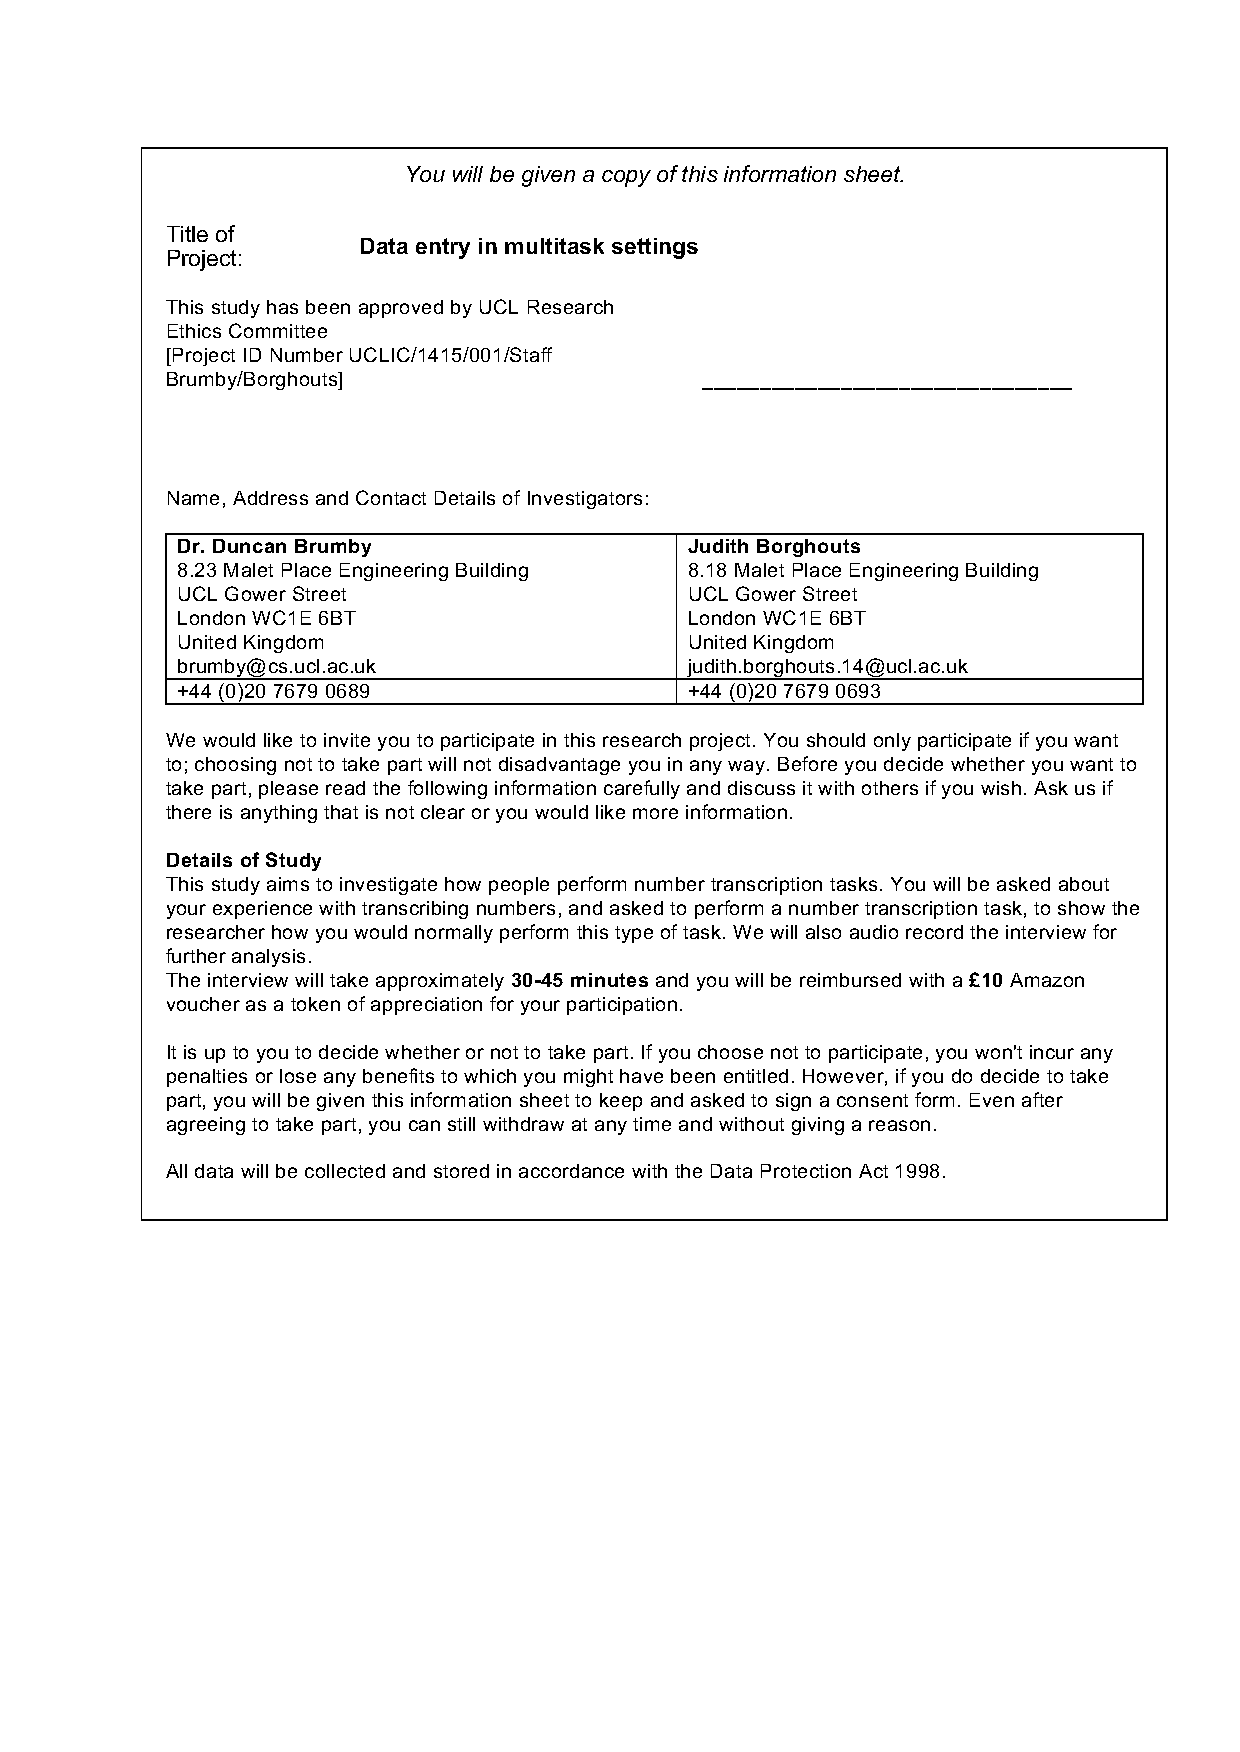
\includegraphics[width=\textwidth,keepaspectratio]{images/Informationsheet.pdf}}
\caption{Information sheet}
\label{fig:informationsheet}
\end{figure} 

\chapter{Consent form}\label{ch:consentform}
The consent form used for Study 1 is shown in Figure \ref{fig:consentform}. 

\begin{figure}[htp] \centering{
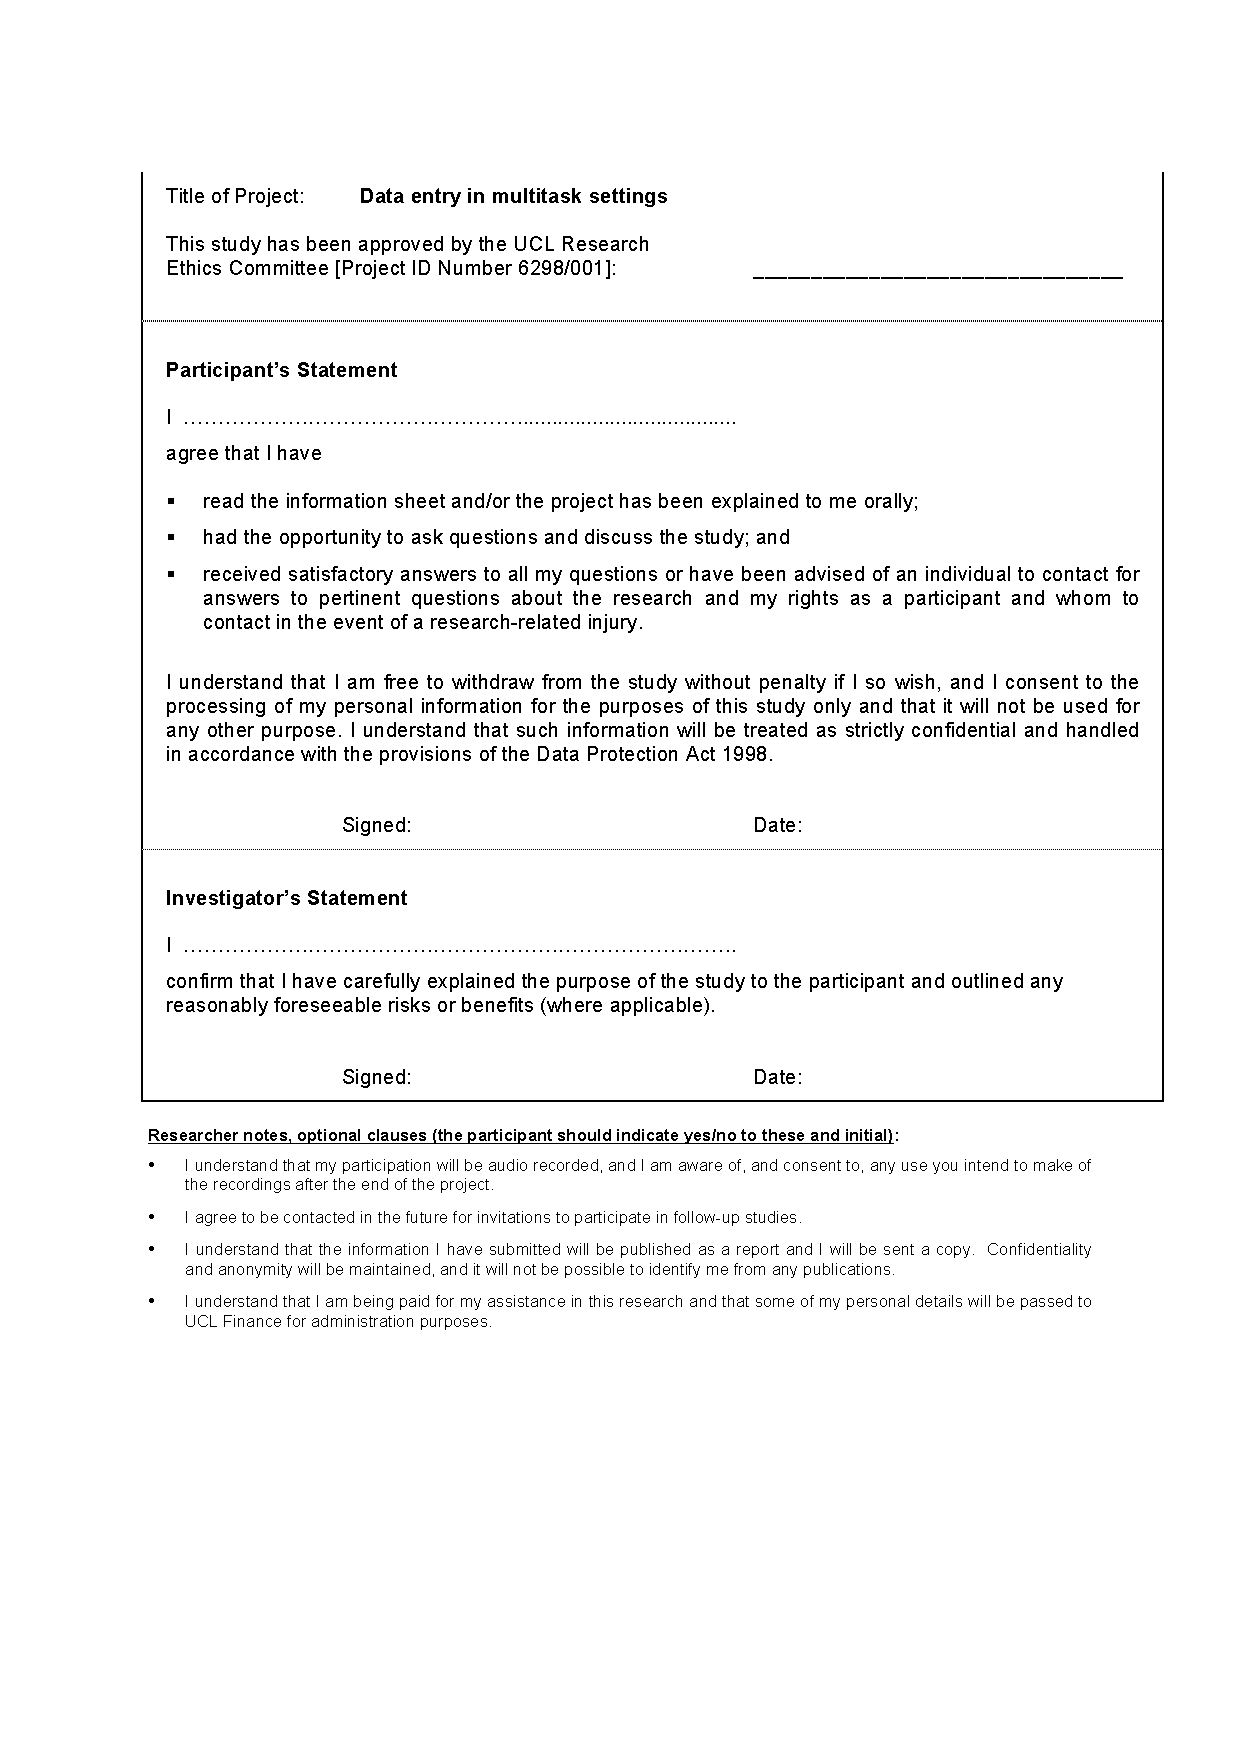
\includegraphics[width=\textwidth,keepaspectratio]{images/Consentform.pdf}}
\caption{Consent form}
\label{fig:consentform}
\end{figure} 

\chapter{Interview script}\label{ch:interviewscript}
The interview script used for Study 1 is given below. This script only served to guide the interview, and does not contain all questions that were asked. Based on what the participant was saying, follow-up questions were asked. 

\subsubsection{Before the interview}
\begin{itemize}
\item 
ensure participant is aware of purpose research 
\item 
explain what will happen
\item 
informed consent
\item 
ask for permission to audio record interview
\end{itemize}
\subsubsection{Work}
\begin{itemize}
\item Tell me something about your work (what do you do)
\item  How many hours per week (full-time/part-time)
\item How long have you been working here (at this company) \item How long have you been doing this type of work
\end{itemize}
\subsubsection{Number entry}
\begin{itemize}
\item  What activities do you do for work that involve transcribing numbers?
e.g. filling in expenses, tax returns, setting up invoices
\item How often do you do this (per day/week)?
\item How many numbers is it roughly that you have to enter?
\item How long do you usually take?
\item What type of numbers? Usually same numbers, or can it be anything?
\item Do you get to enter numbers that are different from your familiar format?
e.g. 2,000 or 2.000; 9/15/14 instead of 15/9/14
\item Do you deal with foreign currencies?
\item Tell me something about how you enter these numbers
\item When do you do these tasks? Immediately when you get them, or save them for later? Morning, afternoon?
\item Does urgency/time pressure influence how you do the task (if so, how)
\item Do you do them in-between other tasks or save a particular part of the day for it?
\item Do you do all tasks all at once, or take rests in between?
(if rests, what do you do? switch to another task, have a coffee, lunch, break, etc.)
\item Do you feel that the way you enter it changes after a while?
e.g. you get better at it so it kind of becomes automatic, or less mentally exhausting? Or is it the opposite, becomes more exhausting?
\item Do you do other things as well during this task
e.g. listening to music, attending to another task
\item Do you sometimes have to briefly store numbers in memory, or calculate them from numbers you already have?
If so, do you use external tools to offload memory?
\item Where do you copy them from? Paper, digital files, combination?
\item Do numbers get checked, to see if they're correct? Do you or anyone else check these numbers?
\item Do you ever get entered numbers from someone else, that you then have to check if they are correct?
\item What is your general experience with transcribing numbers?
e.g. easy, boring, part of the job
\end{itemize}
\subsubsection{Environment}
\begin{itemize}
\item Do you always work in the same environment, or sometimes work in different places, such as at home, or when you're on the train, or working at a cafe? What about number entry tasks?
\item Do you do your work on a desktop, laptop, tablet, anything else? Are some devices harder or easier?
\item How is your desk organized?
\item Do you organise it differently when doing number entry tasks?
\item Do you have notifications on (e.g. e-mail, work-related instant messaging); if you do get new notification, do you attend to it straight away or finish task first?
\item Do you get interrupted in other ways, for example when the phone is ringing, or when a colleague or your boss asks you something? How do you deal with these interruptions? What is your experience with these interruptions?
\item Critical incident: Has there ever been an incident where a mistake in entering a number went undetected, and was discovered later on?
\end{itemize}
\subsubsection{Demonstration}
\begin{itemize}
\item Could you show me the software you use to transcribe numbers?
What is your experience with this system, works well?
(If negative, how do you deal with that? do you use any strategies to make it more optimal for yourself?)
\item Do you feel confident entering the numbers?
\item How do you place your windows?
\item Could you show me how you perform a typical number transcription task (do it how you would normally); if you feel uncomfortable about sharing work data, you can enter any type of numbers, as long as it somewhat resembles data you would normally enter for work
\end{itemize}
\subsubsection{After the interview}
\begin{itemize}
\item Thank participant
\item explain what will happen to their data
\item do they have any more questions
\item clarify when they will be compensated
\item Ask if participant knows any further people who might be suitable and willing to participate
\end{itemize}

\end{document}  